\documentclass[envcountsect,aspectratio=43]{beamer}


\usepackage{pythontex} 
\usepackage{etex}
\usefonttheme[onlymath]{serif}
\usepackage[utf8x]{inputenc}
\usepackage[brazilian]{babel}
\usepackage{amsthm,amssymb}
%\usepackage{graphicx}
\usepackage{wrapfig}
\usepackage{color}
\usepackage{multicol}
\usepackage{makecell}
\usepackage{syntonly}
\hypersetup{colorlinks,linkcolor=,urlcolor=blue}


\usepackage{pgf,tikz}
\usetikzlibrary{calc}
\usetikzlibrary{positioning}
\usetikzlibrary{decorations.pathreplacing}
\usepackage{tkz-euclide}

%\syntaxonly
%\includeonlyframes{int_trig} 
%\includeonlyframes{area-circulo,def_integral} 
%\includeonly{area-circulo,def_integral,int_indefinida_subst,areas,int_partes,int_trig,int_frac_parc,aplicacoes,improprias}%
%\includeonly{def_integral,improprias}%
%\usebackgroundtemplate{\includegraphics{calculus2.eps}}



\usepackage[labelformat=empty]{caption}
\setbeamertemplate{caption}[numbered]{}



\usetheme{Madrid}

\setbeamertemplate{theorems}[numbered]

\newtheorem{nada}{Nada}


\theoremstyle{definition}
\newtheorem{defin}[nada]{Defini\c c\~ao}
\newtheorem{prop}[nada]{Proposi\c c\~ao}

\newtheorem{corol}[nada]{Corol\'ario}

\newtheorem{teo}[nada]{Teorema}

\newtheorem{lema}[nada]{Lema}



\newtheorem{outline}{\timesbold outline rem proof}

\newtheorem{obs}[nada]{Observação}
\newtheorem{afir}{Afirmação}





\makeatletter
\def\th@exercicio{%
	\normalfont % body font
	\def\inserttheoremblockenv{alertblock}  
}
\theoremstyle{exercicio}
\newtheorem*{exer}{
\includegraphics[scale=0.06]{w-brainb.png} Exercício}
\makeatother

\newtheorem{casa}{
\includegraphics[scale=0.035]{w-homework.png} Para Casa}
\makeatother




\makeatletter
\def\th@something{%
	\normalfont % body font
	\def\inserttheoremblockenv{exampleblock}  
}
\theoremstyle{something}
\newtheorem*{exe}{
\includegraphics[scale=0.3]{exemplo.png} Exemplo }
\makeatother

%\setbeamercolor{block title}{bg=cyan, fg=white}

\newtheorem*{casa-comp}{
\includegraphics[scale=0.035]{w-homework-comp.png} Tarefa Computacional}
\makeatother

\makeatletter
\def\th@resp{%
	\normalfont % body font
	\def\inserttheoremblockenv{block}  
}
\theoremstyle{resp}
\newtheorem*{resp}{
\includegraphics[scale=0.01]{White_check.png} Resposta}
\makeatother


\makeatletter
\def\th@desafio{%
	\normalfont % body font
	\def\inserttheoremblockenv{alertblock}  
}

\theoremstyle{desafio}
\newtheorem*{desafio}{
\includegraphics[scale=0.02]{desafio-branco.png} Desafio}
\makeatother


%%%%%%%%%%%%%%%%%%%%%%%%%%%%%%%%%%%%%%%%%%%%%%%%%%%%%%%%%%%%%%%%%%%%%%%%%%%%%%%%%%%%%%%

\newcommand{\cqd}{\hfill \framebox[7pt]{} \mbox{} \medskip}
\newcommand{\dem}{\noindent {\bf Demonstra\c c\~ao:}}
\newcommand{\dest}{\textcolor{blue}}
\newcommand{\R}{\mathbb{R}}
\newcommand{\vect}[1]{\overrightarrow{#1}}
\newcommand{\vt}[1]{\overrightarrow{#1}}
\newcommand{\dt}[1]{\textcolor{blue}{#1}}
\newcommand{\ang}{\widehat}
\newcommand{\n}[1]{\|#1\|}
\newcommand{\pe}[2]{\langle #1,#2\rangle}
\newcommand{\sen}{\operatorname{sen}} 
\newcommand{\tg}{\operatorname{tg}}     
\newcommand{\proj}{\operatorname{proj}}
\newcommand{\pv}[2]{\vt{#1}\times \vt{#2}}
\newcommand{\pmt}[3]{[\vt{#1},\vt{#2},\vt{#3}]}
\newcommand{\ex}{\textcolor{structure}{\large{Exemplo\ \ }}}
\newcommand{\dps}{\displaystyle}
\newcommand{\senh}{\operatorname{senh}}
\newcommand{\tgh}{\operatorname{tgh}}
\newcommand{\sech}{\operatorname{sech}}
\newcommand{\mc}{\textordmasculine\ }

%%%%%%%%%%%%%%%%%%%%%%%%%%%%%%%%%%%%%%%%%%%%%%%%%%%%%%%%%%%%%%%%%%%%%%%%%%%%%%%%%%%%%%%
\definecolor{corcapa}{RGB}{100, 100, 255}



\begin{document}

%\setbeamercovered{transparent}
\title[cálculo II: Integração]{ Cálculo II\\
	\normalsize{Cálculo Integral e Aplicações}}
\author[Reginaldo Demarque]{
		$\displaystyle\int_a^b \textcolor{red}{f(x)}\, dx=\lim_{\|P\|\to 0}\sum_{i=1}^n\textcolor{corcapa}{f(c_i)\Delta x_i}$
		\\
		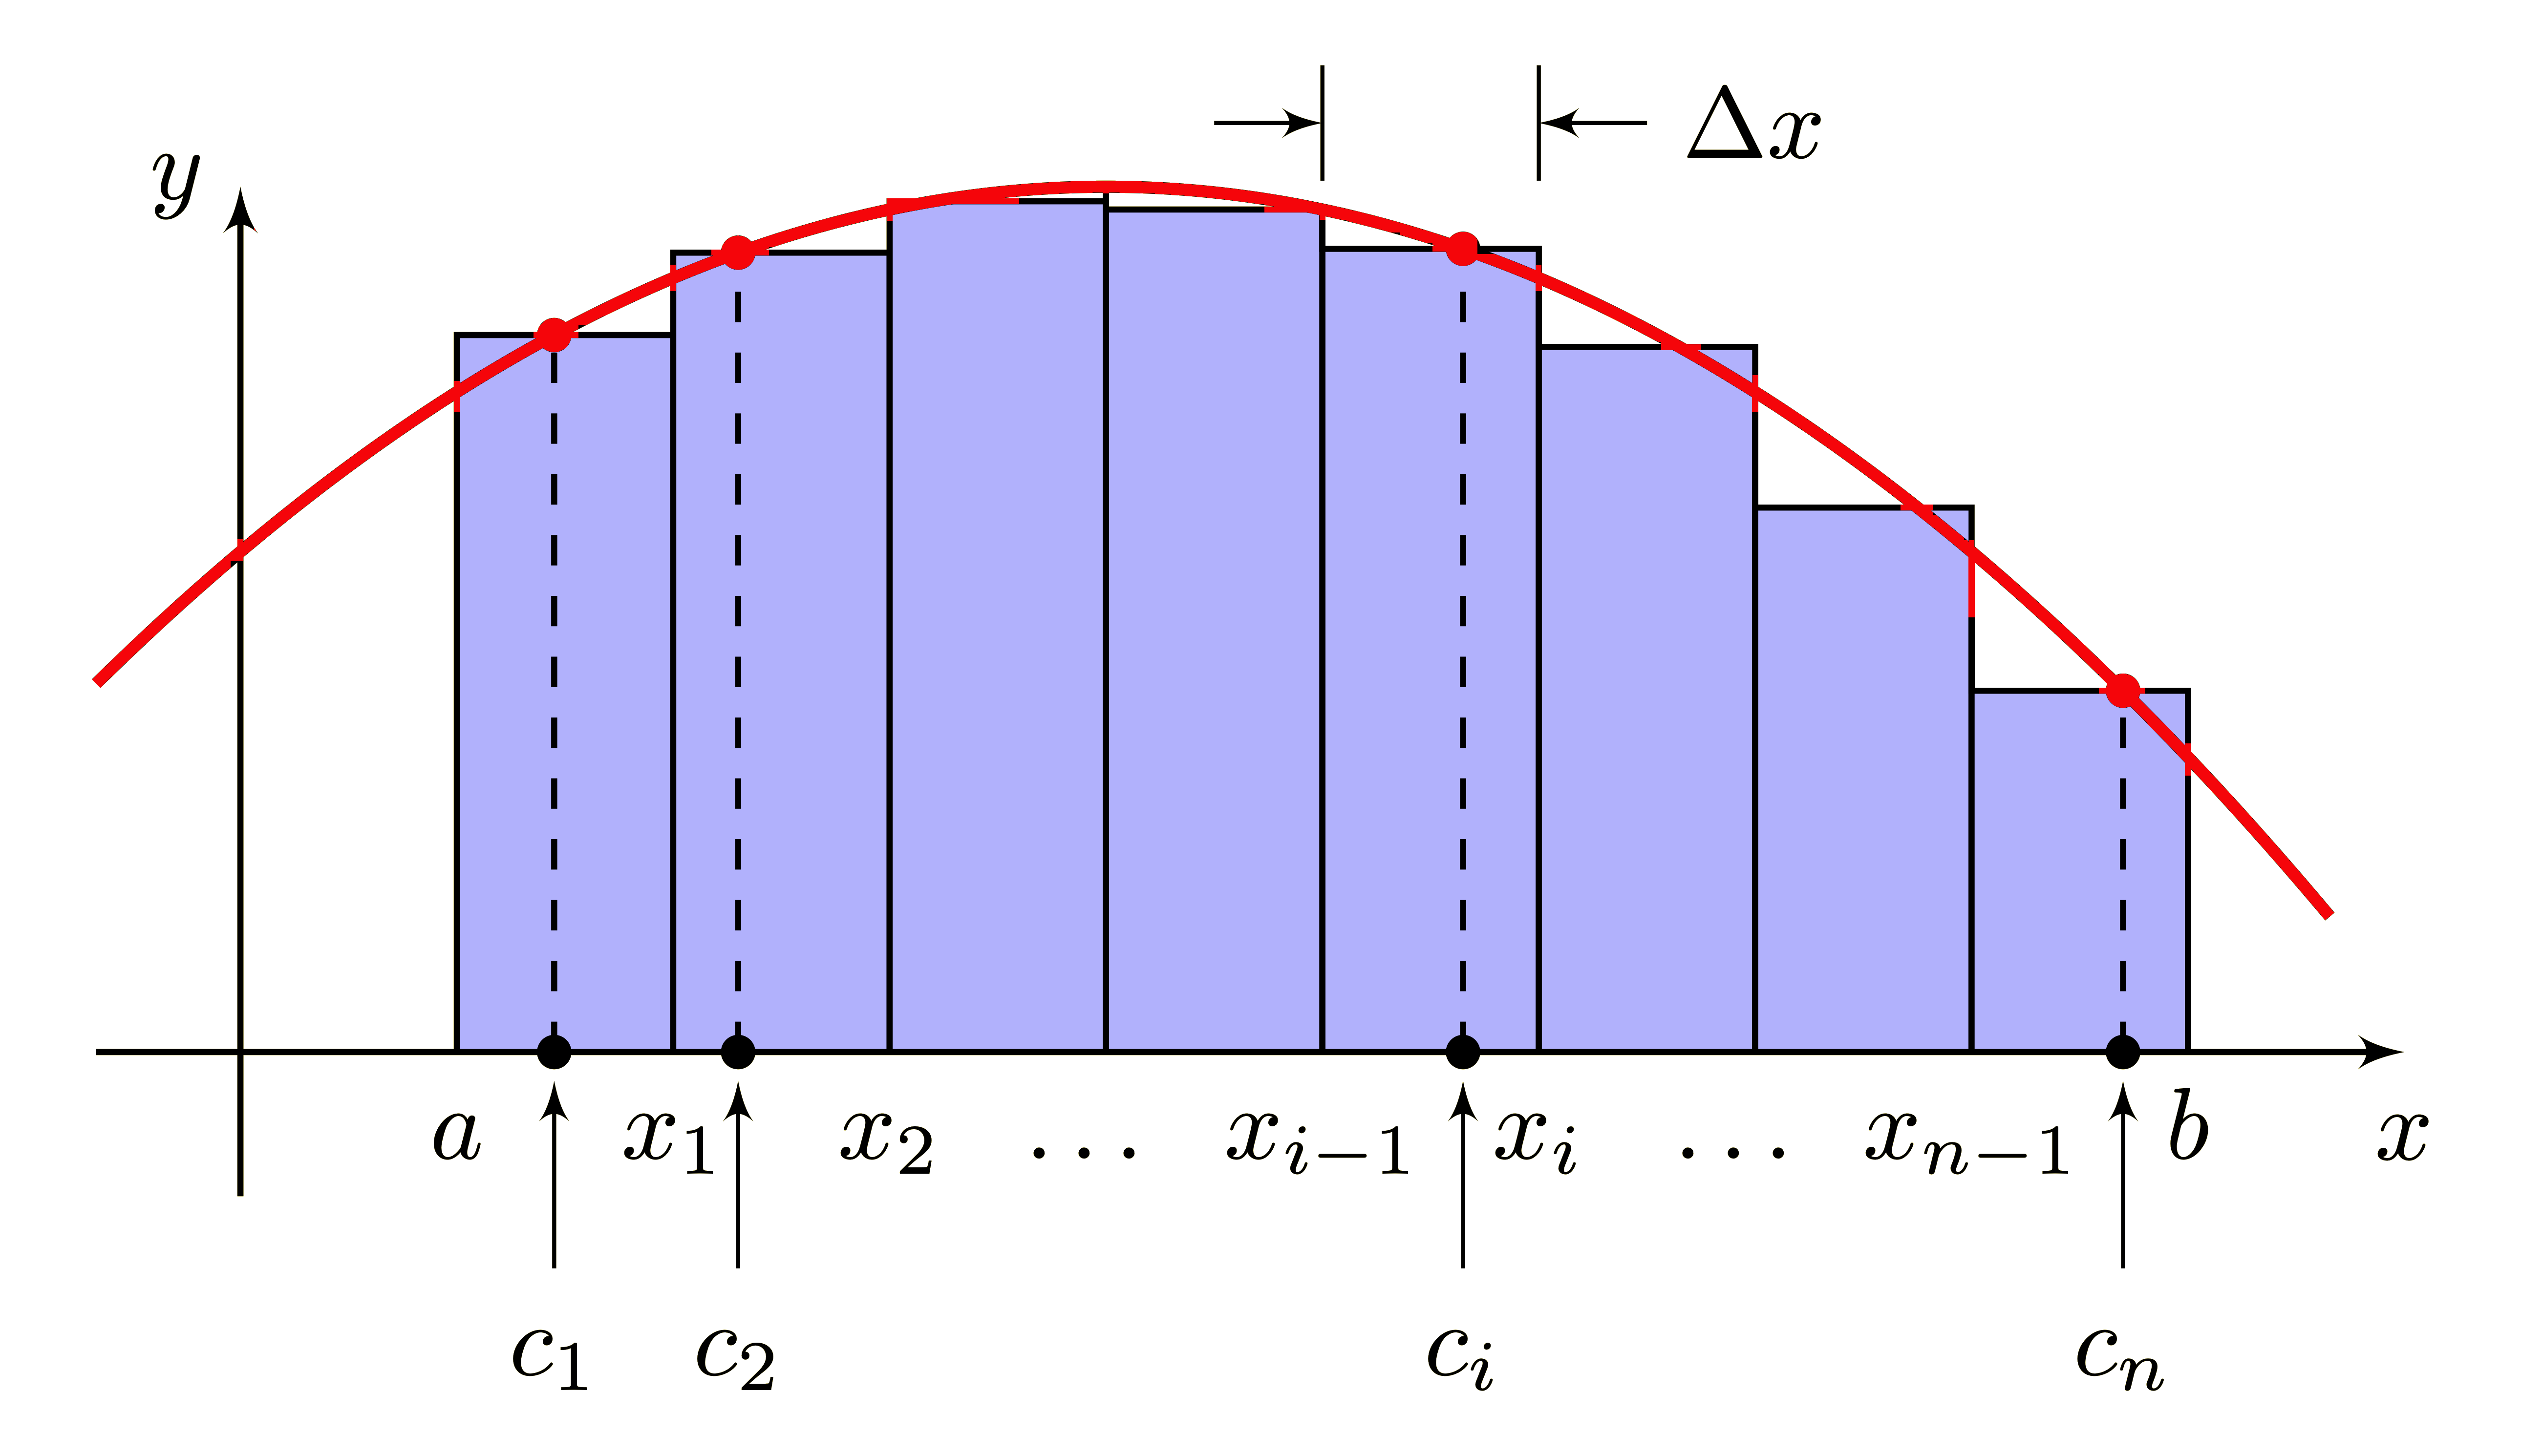
\includegraphics[scale=0.08]{capa2.png}\\
	Prof. Reginaldo Demarque}



%%%%%%%%%%%%%%%%%%%%%%%%%%%%%%%%%%%%%%%%%%%%%%%%%%%%%%%%%%%%%%%%%%%%%%%%%%%%

\logo{
\includegraphics[scale=0.03]{UFF_brasao.png}}

\institute[RCN/UFF]{Universidade Federal Fluminense\\
Instituto de Humanidades e Saúde -- RHS\\
Departamento de Ciências da Natureza -- RCN  \\
\bigskip
%{\color{blue} Atuallizado em \today}
}
\date{{\color{orange} \today}}


\frame{\titlepage}

%%%%%%%%%%%%%%%%%%%%%%%%%% sumario  %%%%%%%%%%%%%%%%%%%%%%%%%%%%%%%%

\frame{
 \frametitle{Sumário}
 \tableofcontents
}



\AtBeginSection[]
{
 \begin{frame}

  \frametitle{Sumário}
  \tableofcontents[currentsection]

 \end{frame}
}


\section{A Integral}

\subsection*{Um pouco de história}

\begin{frame}[label=area-circulo]{A origem do Cálculo Integral}
	Na segunda metade do século XVII, \textcolor{blue}{Newton} na Inglaterra e \textcolor{blue}{Leibniz} na Alemanha mudaram o curso da matemática para sempre. Ele pegaram uma colcha de retalhos soltas de ideias sobre movimento e curvas e transformaram isso no cálculo. 


	\begin{center}
				\begin{minipage}{0.4\textwidth}
\begin{center}
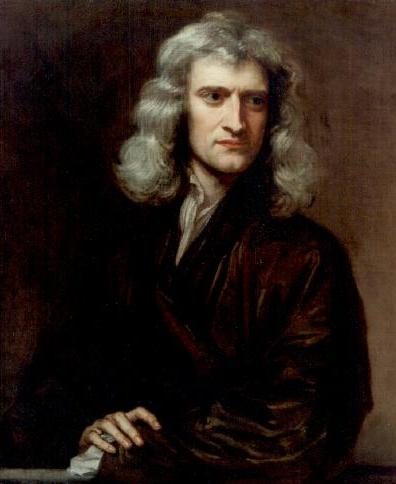
\includegraphics[scale=0.35]{newton.jpg}

{\scriptsize 	Isaac Newton\\ 1643-1727 }
\end{center}
	\end{minipage}	
	\begin{minipage}{0.4\textwidth}
		
\begin{center}
	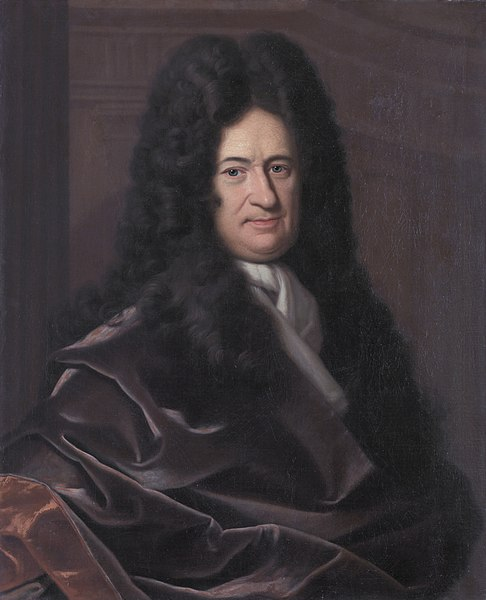
\includegraphics[scale=0.2]{leibniz.jpg}

			{\scriptsize Gottfried Wilhelm Leibniz \\  1646-1716 }
\end{center}
	\end{minipage}
	\end{center}
\end{frame}



\begin{frame}[label=area-circulo]{O Precursor do Cálculo}
	Muitos historiadores acreditam que  o verdadeiro precursor do cálculo foi \textcolor{blue}{Arquimedes}. Ele aperfeiçoou o método da exaustão de Eudoxus para  encontrar áreas de figuras planas. 
\medskip

Arquimedes é considerado o maior matemático da antiguidade. Segundo a lenda, foi morto por um soldado romano durante a tomada da cidade enquanto estudava um diagrama geométrico na areia.
\smallskip

	\begin{minipage}{0.3\linewidth}
		
	\begin{center}
		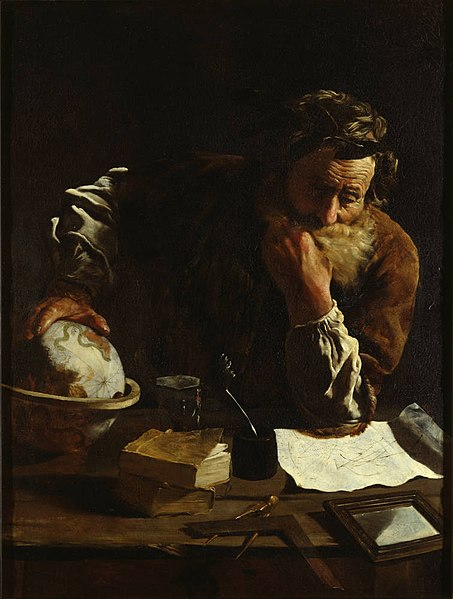
\includegraphics[scale=0.15]{arquimedes.jpg}
		
		{\tiny Arquimedes de Siracusa \\ 287-212 BCE. \\ Pint. Domenico Fetti (1620)}
	\end{center}
	
	\end{minipage}
\begin{minipage}{0.65\linewidth}
	 
	
	Em seu livro \textcolor{blue}{A Medida do Círculo} ele mostrou que o valor exato do número $\pi$   está entre \textcolor{red}{223/71 e 22/7}, ou seja, estaria aproximadamente entre \textcolor{red}{3,1408 e 3,1429}, aproximação que obteve inscrevendo e circunscrevendo o círculo em um polígono regular de \textcolor{red}{96 lados}. Usando este método ele foi capaz de calcular o volume da esfera, o volume e a área do cone, o volume obtido por revolução de qualquer segmento de uma parábola ou hipérbole.
\end{minipage}
\end{frame}


\begin{frame}[label=area-circulo]{Método da Exaustão de Eudoxus}


\begin{center}
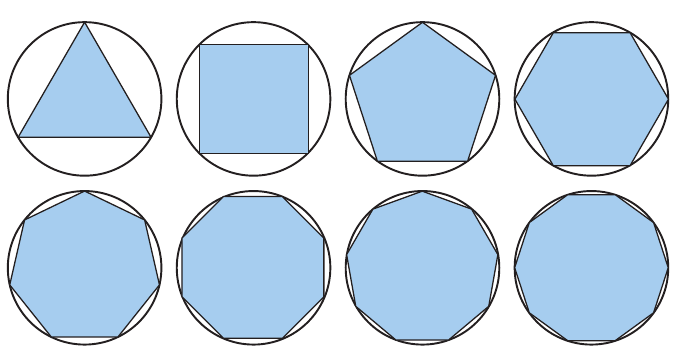
\includegraphics[scale=.5]{figuras/circulo-area.png}
\end{center}

\end{frame}

\begin{frame}[label=area-circulo,fragile=singleslide]{Polígonos Inscritos}
Na tabela abaixo temos a área $A_n$ de um polígono regular de $n$ lados inscrito em um círculo de raio 1.
\medskip

%	\begin{scriptsize}
\begin{center}
		\begin{pycode}
import sympy as sp

#dados iniciais
m=6 #começando com um hexágono regular
l=1 #lado do hexágono

#aproximação da área usando um polígono de n lados inscritos no círculo
print(r"\begin{tabular}{c|c|c}")
print(r" n &  $A_n$ & erro \\ \hline")
for n in range(10):
 h=sp.sqrt(1-l**2/4) #altura de cada triângulo dado o lado
 l=sp.sqrt(l**2/4+(1-h)**2) #lado do polígono da próxima iteração
 m=2*m  #número de lados do polígono seguinte  
 p=m*l  #perímetro do polígono de n lados 
 c=p/2
 n+=1
 print(r" ",m,"&",p/2,"&",sp.pi.evalf()-c,r"\\")
print(r"\end{tabular}")
		\end{pycode}
\end{center}
%	\end{scriptsize}
\end{frame}




\begin{frame}[label=area-circulo]{A ideia da integral}


\begin{center}
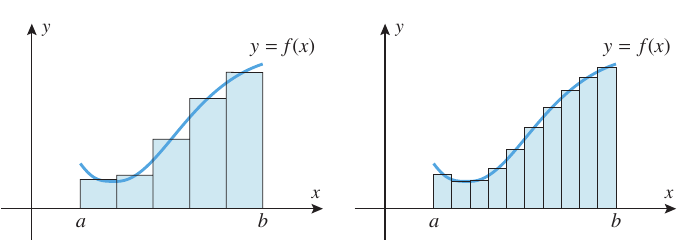
\includegraphics[scale=.55]{figuras/soma-rieman1.png}

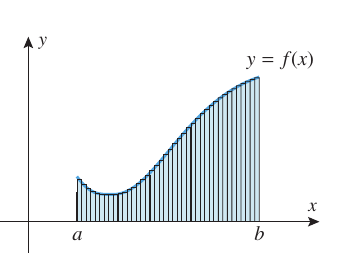
\includegraphics[scale=.55]{figuras/soma-rieman2.png}
\end{center}

\end{frame}




\subsection*{Notação Sigma}


\begin{frame}[label=def_integral]
\frametitle{Notação Sigma }
\begin{small}
\noindent A notação sigma permite expressar uma soma com muitos termos em uma forma compacta.
$$\sum_{k=1}^na_k=a_1+a_2+a_3+\cdots+a_{n-1}+a_n$$

\begin{itemize}
\item O símbolo $\sum$ é chamado de somatório. Ele é a letra grega sigma maiúscula correspondente ao nosso S significa.

\item $k$ é o índice do somatório.

\item $a_k$ é o termo geral da soma.

\item 1 é o índice inferior e $n$ é o índice superior.

\end{itemize}

\end{small}

\end{frame}



\begin{frame}[label=def_integral]
\begin{exe}
\begin{enumerate}
\item $\dps\sum_{k=1}^4k^2=1+4+9+16=30$
\item $\dps\sum_{k=1}^5(-1)^k k=?$
\end{enumerate}
\end{exe}

\end{frame}

\subsection*{Somas de Riemann}

\begin{frame}[label=def_integral]
\frametitle{Partições de um intervalo }

\uncover<1->{Dado $[a,b]$ um intervalo fechado da reta,  o seguinte conjunto
\[P=\{x_0,x_1, \ldots, x_{n-1}, x_n\},\]
onde $a=x_0< x_1<\ldots < x_{n-1}< x_n=b$, é dito uma \dt{partição} de $[a,b]$.}
\medskip

\uncover<1->{Seja $\Delta x_i=(x_i-x_{i-1})$ o comprimento do intervalo $[x_{i-1},x_i]$ para todo $i=1,\ldots,n$. }

Um conjunto $\textcolor{blue}{\{c_1,c_2,\ldots,c_n\}}$, onde $\textcolor{blue}{c_i}\in[x_{i-1},x_i]$ é dito um \dt{pontilhamento} da partição $P$. Uma partição $P$ a qual escolhemos um pontilhamento  é dita uma \dt{partição pontilhada} e é denotada por $P^\ast$.
\medskip


%\uncover<1->{Definimos a \dt{norma } de uma partição $P$, denotada por $\|P\|$, como o maior dos $\Delta x_i$ com $i=1,\ldots,n$.}

\end{frame}


\begin{frame}[label=def_integral]
\frametitle{Somas de Riemann }

Seja $\textcolor{red}{f:[a,b]\to \R}$ uma função limitada e $P=\{x_0,x_1,\ldots,x_n\}$ uma partição qualquer de $[a,b]$.

\medskip


\uncover<1->{A soma
$$R(\textcolor{red}{f},P^\ast)=\sum_{i=1}^n\textcolor{red}{f}(\textcolor{blue}{c_i})\Delta x_i,$$
é dita uma \dt{soma de Riemann para f no intervalo [a,b]}.}
\medskip


\begin{center}
	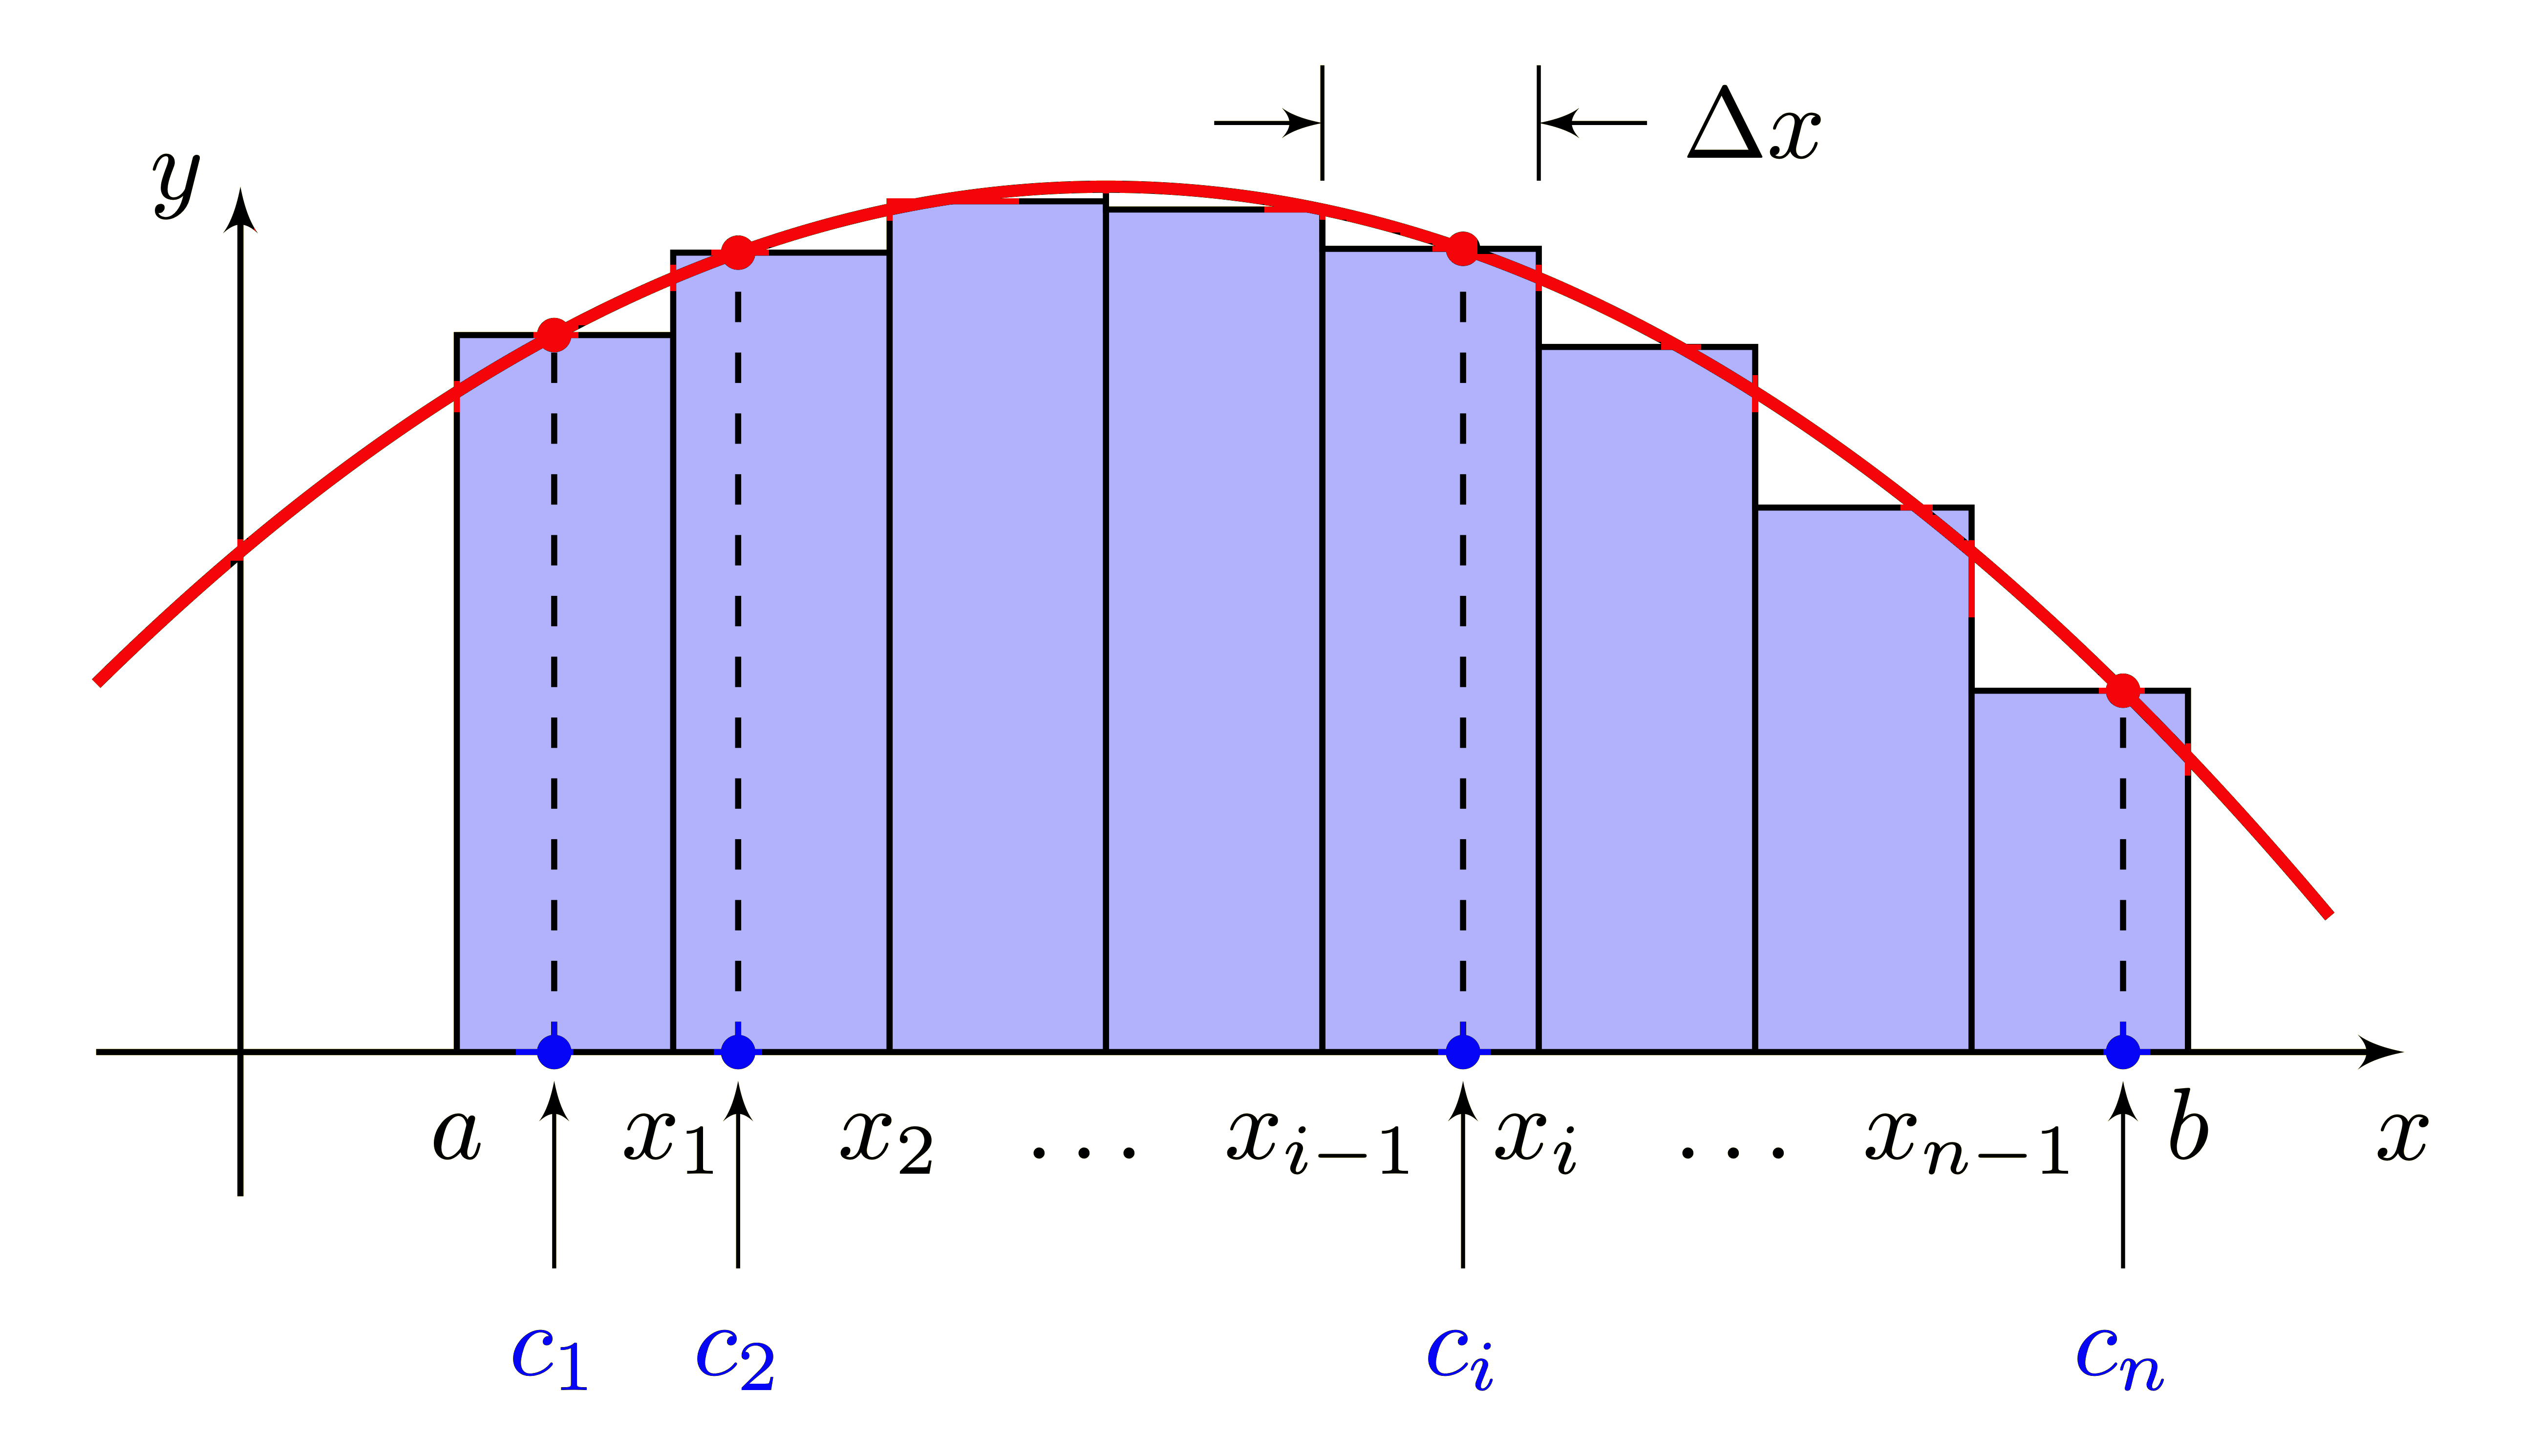
\includegraphics[scale=0.15]{capa3.png}
\end{center}


\end{frame}


\begin{frame}[label=def_integral]{Somas inferiores}
	\begin{itemize}
		\item $f:[a,b]\to \R$ contínua e $m_i=\dps\min_{[x_{i-1},x_i]}f(x)$
		
		\item $s(f,P)=\dps\sum_{i=1}^{n}m_i\Delta x_i$ \dt{somas inferiores } de $f$ em relação a $P$.
	\end{itemize}
	
%\uncover<1->{Dados uma função $f:[a,b]\to \R$ contínua e uma partição $P$  do intervalo $[a,b]$, definimos $m_i$ e $M_i$ como sendo o menor e o maior valor de $f(x)$ quando $x$ varia no intervalo $[x_{i-1},x_i]$, respectivamente.}
%\medskip
%
%\uncover<1->{Definimos ainda como $s(f,P)=\dps\sum_{i=1}^{n}m_i\Delta x_i$ e $S(f,P)=\dps\sum_{i=1}^{n}M_i\Delta x_i$ as \dt{somas inferiores } e \dt{somas superiores} de $f$ em relação à partição $P$, respectivamente.}
%\medskip

\begin{center}
	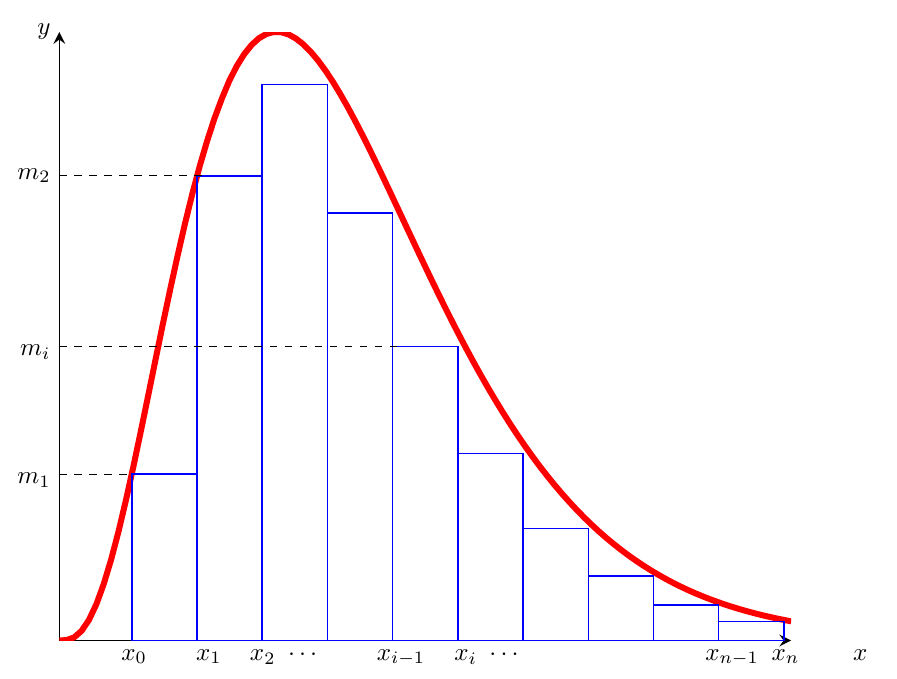
\includegraphics[scale=0.3]{som-inf.png}
\end{center}
\end{frame}


\begin{frame}[label=def_integral]{Somas Superiores}
	\begin{itemize}
		\item $f:[a,b]\to \R$ contínua e $M_i=\dps\max_{[x_{i-1},x_i]}f(x)$
		
		\item $S(f,P)=\dps\sum_{i=1}^{n}M_i\Delta x_i$ as \dt{somas superiores} de $f$ em relação a $P$.
	\end{itemize}
	\begin{center}
		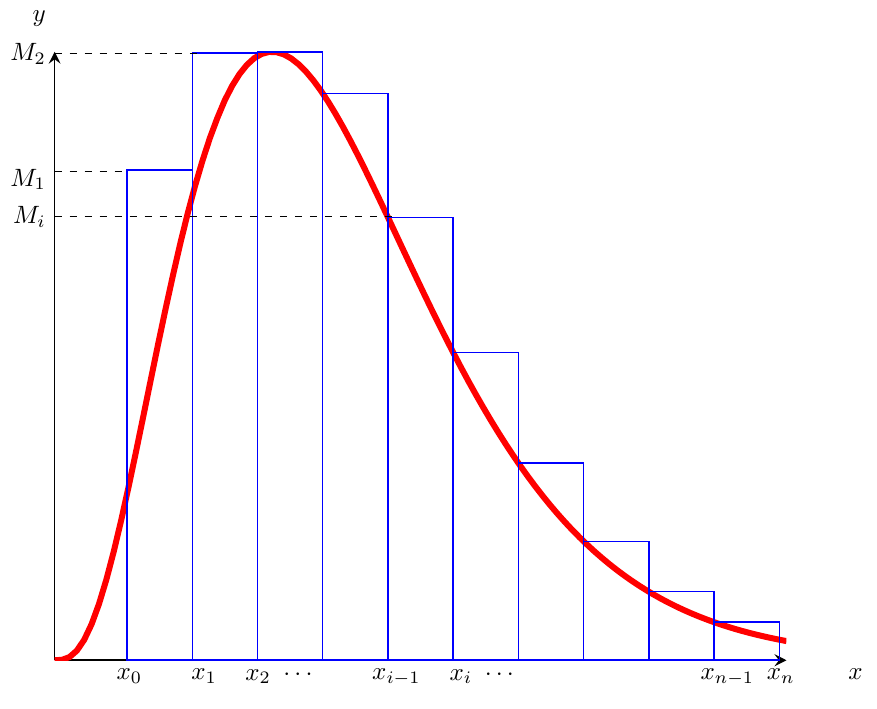
\includegraphics[scale=0.3]{som-sup.png}
	\end{center}
\end{frame}

\begin{frame}[label=def_integral]
\uncover<1->{\begin{exe}
 Encontre a área abaixo do gráfico de $f(x)=x^2$ quando $x\in[0,10]$.
\end{exe}}

\only<1>{
\begin{center}
	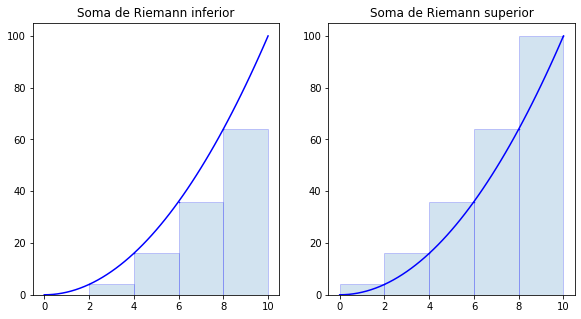
\includegraphics[scale=0.5]{int-rem1.png}
\end{center}

Partição com  {\color{red} 5 subintervalos} de mesmo comprimento.
\[s(f,P)=240\leq A\leq 440=S(f,P)\]}

\only<2>{
	\begin{center}
		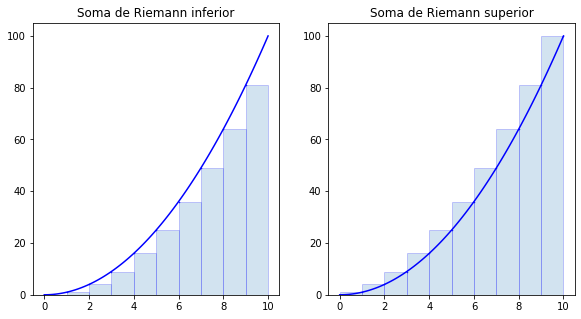
\includegraphics[scale=0.5]{int-rem2.png}
	\end{center}
	
	Partição com  {\color{red} 10 subintervalos} de mesmo comprimento.
	\[s(f,P)=285\leq A \leq 385=S(f,P)\]}

\only<3>{
	\begin{center}
		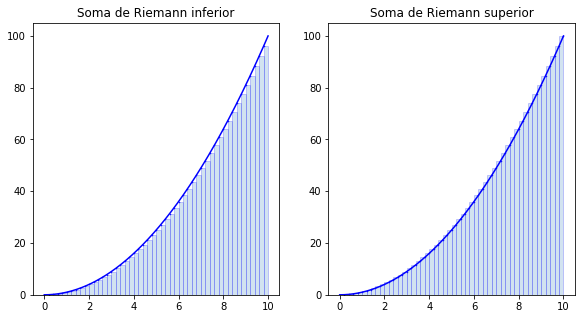
\includegraphics[scale=0.5]{int-rem3.png}
	\end{center}
	
	Partição com {\color{red} 50 subintervalos} de mesmo comprimento.
	\[s(f,P)=323\leq A \leq 343=S(f,P)\]}
\only<4>{
	\begin{center}
		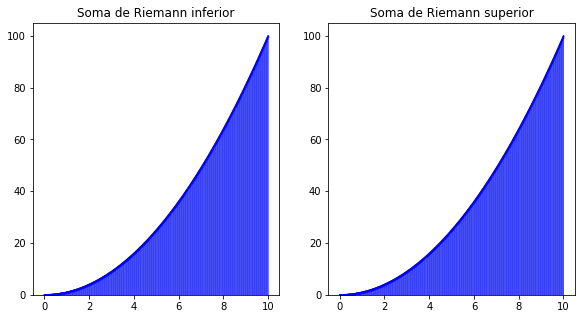
\includegraphics[scale=0.5]{int-rem4.png}
	\end{center}
	
	Partição com  {\color{red} 1000 subintervalos} de mesmo comprimento.
	\[s(f,P)=332.8335\leq A \leq  S(f,P)=333.8335\]}
%\end{small}

\end{frame}

\begin{frame}
\begin{casa}
Mostre que para $f(x)=x^2$, com $x\in[0,10]$, se $P$ é uma partição com $n$ subintervalos de mesmo comprimento, isto é, $\Delta x_i=10/n$, para todo $i=1,2,\ldots, n$, então
\[s(f,P)=\frac{1000}{n^3}\sum_{i=1}^{n}(i-1)^2\]
e
\[S(f,P)=\frac{1000}{n^3}\sum_{i=1}^{n}i^2.\]

Aplique o limite quando $n\to+\infty$ e conclua que a área abaixo do gráfico de $f$ é $\frac{1000}{3}$
\end{casa}
\end{frame}




\subsection*{Definição de Integral}
\begin{frame}[label=def_integral]


\uncover<1->{\begin{defin}Dizemos que uma função $f:[a,b]\to \R$ limitada é \dt{integrável em  $[a,b]$} quando existe um número real $I$ tal que 
$$\lim_{\|P\|\to 0}\sum_{i=1}^nf(c_i)\Delta x_i=I,$$
qualquer que seja a partição $P^\ast$. Em caso afirmativo dizemos que  $I$  é a \dt{integral} de $f$ em $[a,b]$ e o denotamos por $\int_a^bf(x)dx.$
\end{defin}}



\begin{center}
	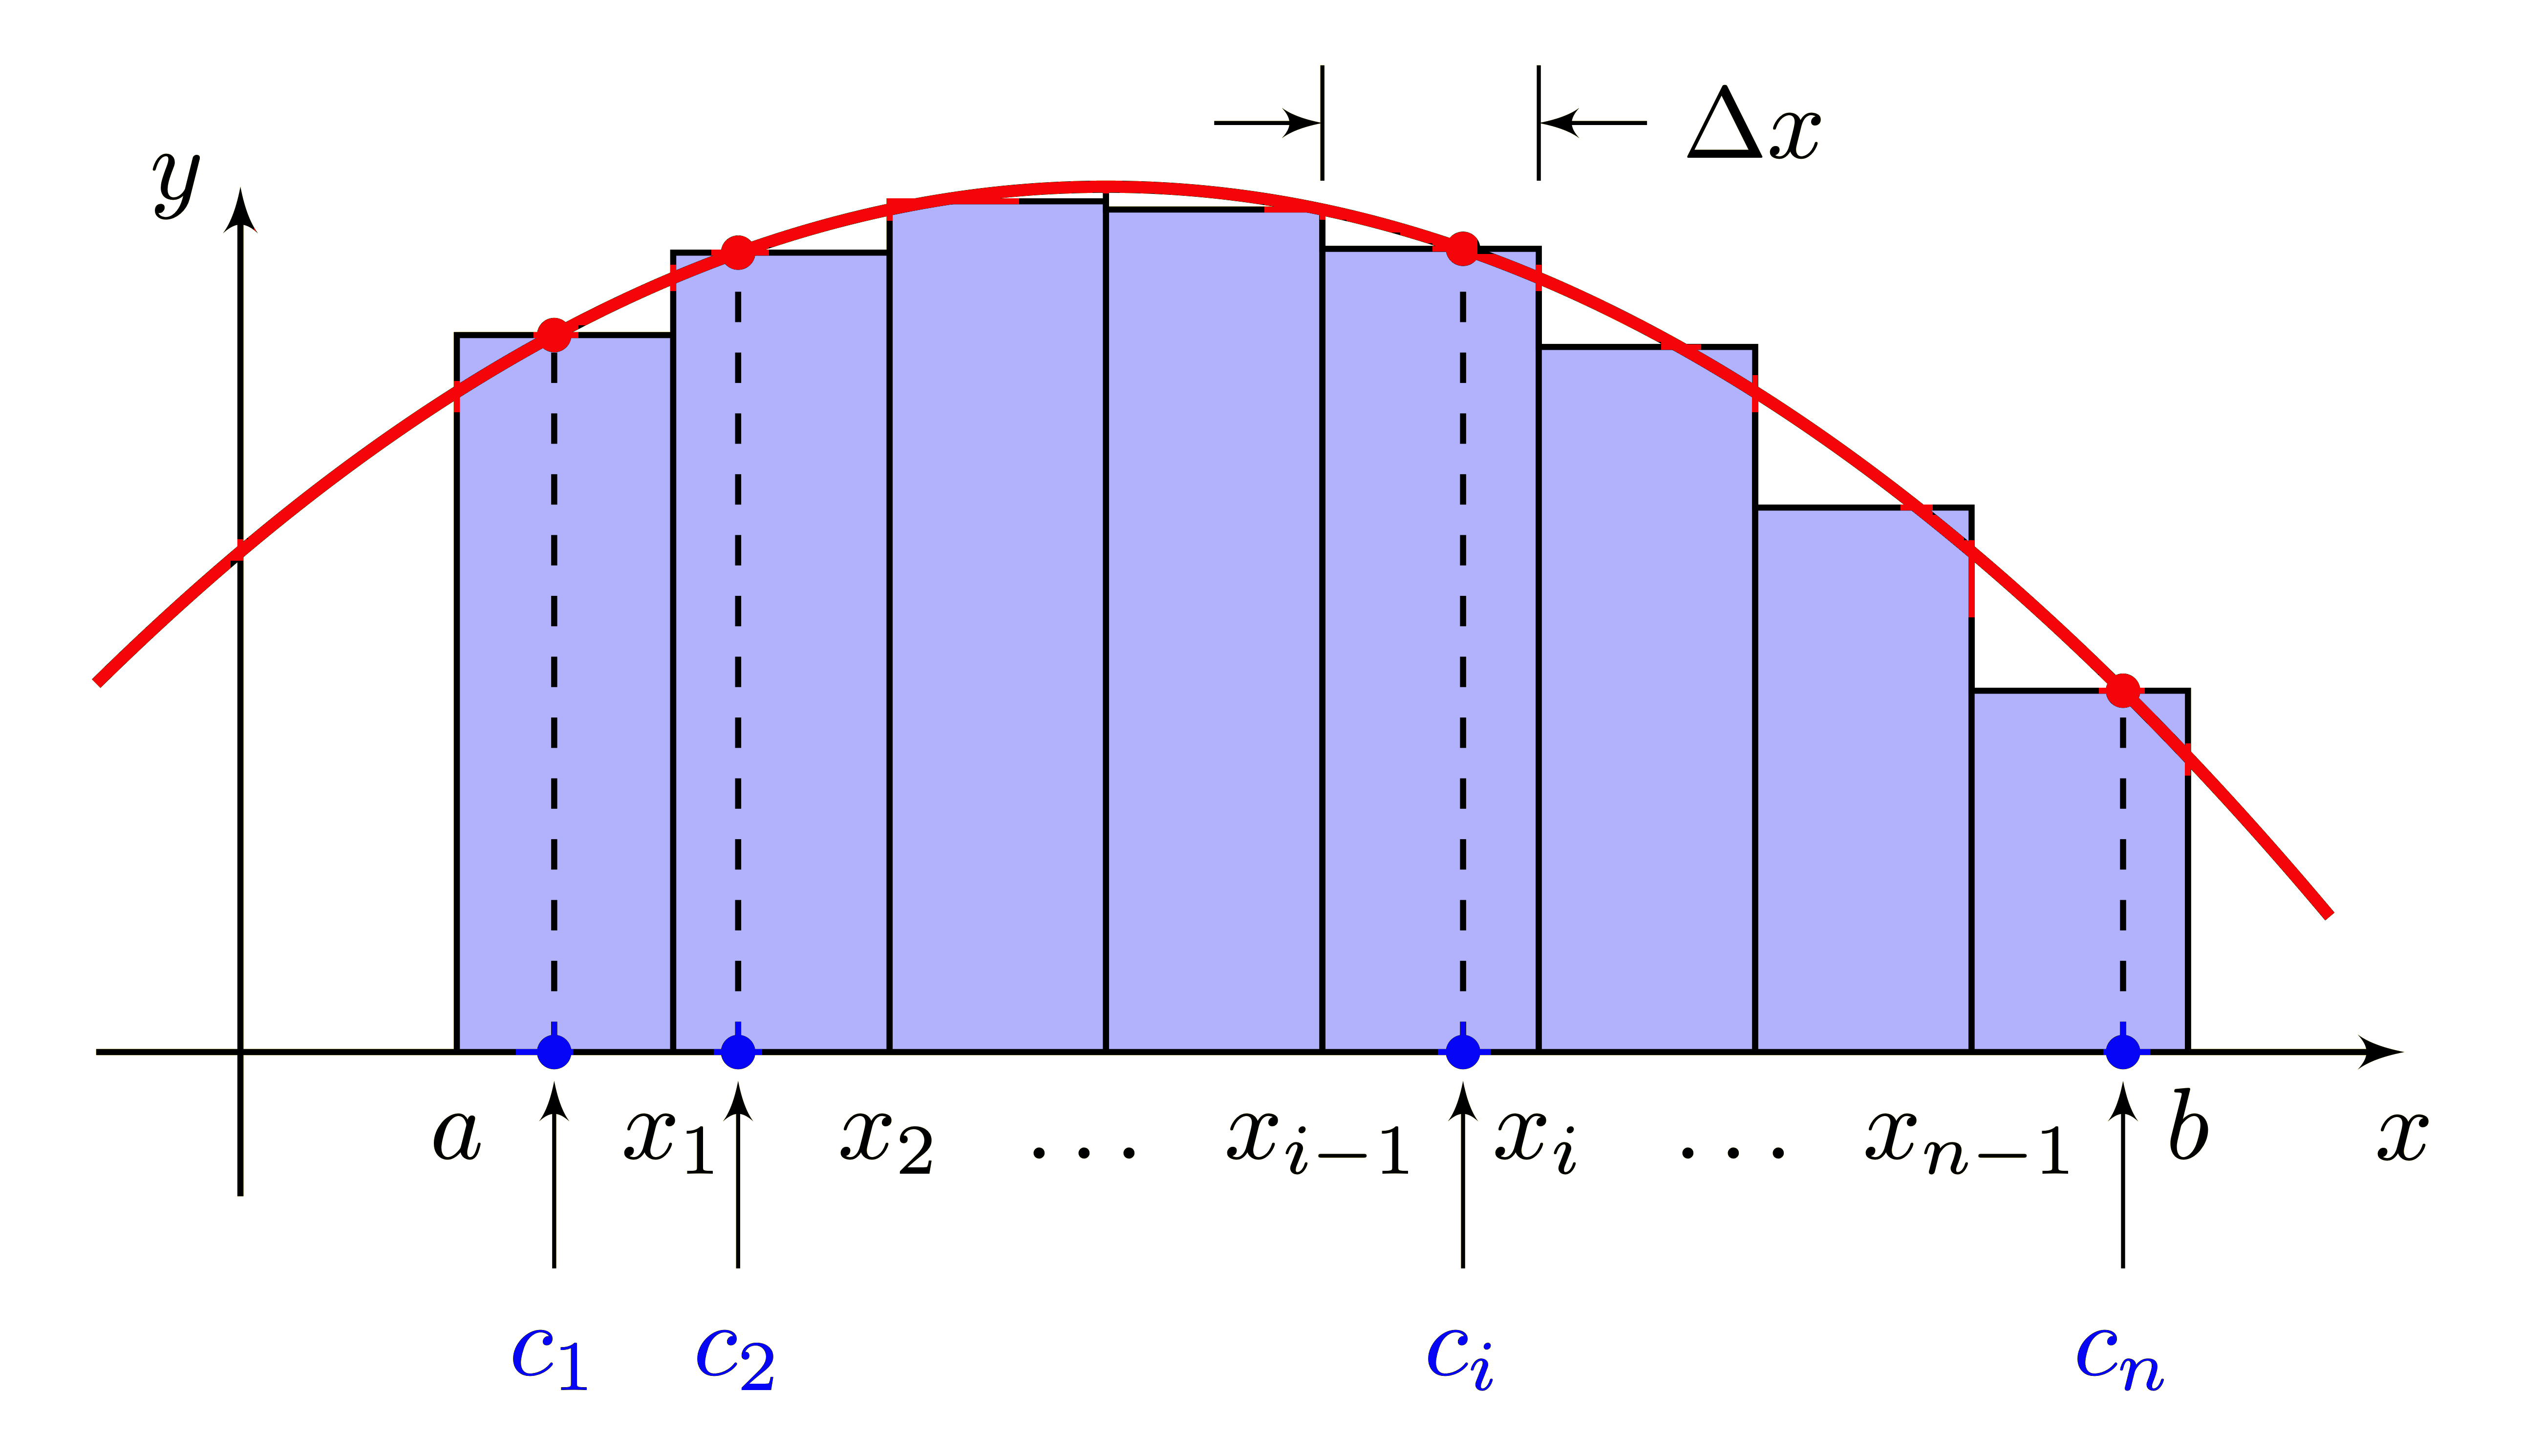
\includegraphics[scale=0.15]{capa3.png}
\end{center}
\end{frame}

\begin{frame}[label=def_integral]
\begin{block}{ }
O símbolo $\int$ de integral, que é um S alongado, foi introduzido por Leibniz em 1675. Leibniz não só tinha uma notável habilidade para construir notações; também criou termos como abscissa, ordenada, coordenada, eixo de coordenadas e função.  Quem primeiro usou a palavra ``integral" foi Jacob Bernoulli, em 1690.
\end{block}

\begin{block}{Área}
Pela construção,  quando $f(x)\geq 0$ para todo $x\in [a,b]$, vimos que a área abaixo do gráfico da função e acima do eixo $x$ é dada pela integral, isto é,
\[\text{Área}=\int_a^bf(x)\,dx\]
\end{block}
\end{frame}





\subsection*{Teorema Fundamental do Cálculo}




\begin{frame}[label=def_integral]
\frametitle{Teorema Fundamental do Cálculo }
\begin{small}


\uncover<1->{\begin{teo} Se $f:[a,b]\to \R$  é contínua e $F$ é uma primitiva de $f$, então
\begin{equation} \label{ident_TFC}\int_a^bf(x)dx=F(b)-F(a)\end{equation}
\end{teo}}

\uncover<1->{\begin{exe}
\begin{multicols}{2}
\begin{enumerate}
\item $\dps\int_0^1 x^2dx$
\item $\dps\int_0^1 x^3dx$
\item $\dps \int_a^b x^n dx$
\item $\dps\int_0^\pi \sen x\ dx$\\
\end{enumerate}
\end{multicols}
\end{exe}}



\end{small}
\end{frame}




\begin{frame}[label=def_integral]
\begin{small}

\uncover<1->{\begin{corol}\label{corol_TFC} Se $f:[a,b]\to \R$  é contínua, então
\begin{equation} 
\frac{d}{dt}\int_a^t f(x)dt=f(t), \forall t\in [a,b].
\end{equation}
\end{corol}}
\uncover<2->{
\begin{quote}
``O Teorema Fundamental do Cálculo é inquestionavelmente o mais importante do cálculo e realmente é um dos grandes feitos da mente humana. Antes de sua descoberta, desde os tempos de Eudóxio e Arquimedes até os de Galileu e Fermat, os problemas de encontrar áreas, volumes e comprimentos de curvas eram tão difíceis que somente um gênio poderia fazer frente ao desafio. Agora, porém, armado com o método sistemático que Leibniz e Newton configuraram a partir do Teorema Fundamental, veremos nos capítulos a seguir que esses problemas desafiadores são acessíveis para todos nós.''

\begin{flushright}
J. Stewart, Cálculo Vol. 1.
\end{flushright}
\end{quote}
 }

\end{small}
\end{frame}


\subsection*{Propriedades da Integral}
\begin{frame}[label=def_integral]
\frametitle{Propriedades da Integral }
\begin{teo} Se $f$ {\color{blue}for contínua em $[a,b]$}, ou tiver {\color{red}apenas um número finito de descontinuidades} do tipo saltos, então $f$ é integrável em $[a,b]$.
\end{teo}

\uncover<1->{Sejam $f$ e $g$ funções integráveis no intervalo $[a,b]$ e $k\in\R$ uma constante.

\begin{enumerate} 

\item $\dps \int_a^b k\ dx=k(b-a)$
\item $\dps \int_b^a f(x)dx:=-\int_a^b f(x)dx$ 
\item $\dps \int_a^a f(x)dx=0$
\end{enumerate} }

\end{frame}


\begin{frame}[label=def_integral]


\begin{enumerate}
\setcounter{enumi}{3}
\item $\dps \int_a^b kf(x)dx=k\int_a^b f(x)dx$
\item $\dps \int_a^b f(x)+g(x)dx=\int_a^b f(x)dx+\int_a^b g(x)dx$
\item $\dps \int_a^c f(x)dx+\int_c^b f(x)dx=\int_a^b f(x)dx$
\item  Se $f\leq g$, então $\dps \int_a^b f(x)dx\leq \int_a^b g(x)dx$
\end{enumerate}

\end{frame}




\begin{frame}[label=def_integral, fragile=singleslide]{Usando Python}
%\begin{small}
\begin{block}{ }
\begin{pyverbatim}
import sympy as sp

x = sp.symbols('x') #variável
f=sp.sin(x) #função

sp.integrate(f,(x,0,sp.pi)) #integral definida
\end{pyverbatim}
\end{block}
%\end{small}
\begin{pycode}
import sympy as sp

x = sp.symbols('x') #variável
f=sp.sin(x) #função
intf2=sp.integrate(f,(x,0,sp.pi)) #integral definida
intf=sp.integrate(f,x)
\end{pycode}

\[\dps \int_0^\pi \py{sp.latex(f)}\, dx=\py{sp.latex(intf)}\bigg\vert_{x=0}^{x=\pi}={\color{blue}\py{sp.latex(intf2)}}.\]
\end{frame}




\begin{frame}[label=def_integral]
	\begin{casa}
 Calcule as integrais
\begin{enumerate}[a]
	\item $\dps\int_1^3\frac{1}{x^2}\,dx$
	\item $\dps\int_1^2\frac{1}{x}\,dx$
	\item $\dps\int_{1}^{4} \frac{2x^
	3+x^3\sqrt{x}-1}{x^3}\,dx$
\end{enumerate}
	\end{casa}

\begin{casa}
Determine área da região limitada que está acima do eixo $x$ e abaixo do gráfico da função $y=x^3-x$.
\end{casa}
\end{frame}


\subsection*{Integral indefinida}
\begin{frame}
\frametitle{ Integral indefinida}
\begin{small}

\uncover<1->{A \dt{integral indefinida} de $f$ em relação a $x$ é o conjunto de todas as primitivas de uma função $f$ e denotamos da seguinte forma
$$\int f(x)dx.$$
O símbolo $\int$ é dito \dt{sinal de integração}, $f$ é dita \dt{integrando} da integral e $x$ é a \dt{variável de integração.}}

\uncover<2->{\begin{exe} Encontre as integrais indefinidas
$$\int \frac{1}{x}dx,\ \ \int e^x\ dx, \ \ \int\frac{1}{1+x^2}dx, \ \ \int \sec^2 dx.$$
\\

\end{exe}}

\end{small}
\end{frame}


\begin{frame}[fragile=singleslide]{Usando Python}
%\begin{small}
\begin{block}{ }
\begin{pyverbatim}
import sympy as sp

x = sp.symbols('x') #variável
f=1/x #função
g=1/(1+x**2) #função
intf=sp.integrate(f,x) #integral indefinida
intg=sp.integrate(g,x) #integral indefinida
\end{pyverbatim}
\end{block}
%\end{small}
\begin{pycode}
import sympy as sp
x = sp.symbols('x') #variável
f=1/x #função
g=1/(1+x**2) #função
intf=sp.integrate(f,x) #integral indefinida
intg=sp.integrate(g,x) #integral indefinida
\end{pycode}

\[\dps \int \frac{1}{x}\, dx=\py{sp.latex(intf)}+C,\ \dps \int \frac{1}{1+x^2}\, dx=\py{sp.latex(intg)}+C.\]

\begin{alertblock}{Observação}
Neste curso, reservaremos a notação $\log(x)$ para o logarítmo na base $e$, isto é, 
$\log(x)=\log_e(x)$. Veja a justificativa em \href{https://reginaldodr.github.io/academic/posts/notacao-log/notacao-log.html}{\beamergotobutton{Link}}
\end{alertblock}

\end{frame}


%\begin{frame}{Aplicações}
%
%\begin{exampleblock}{Queda livre de corpos}
%Consideremos um corpo de massa \textcolor{blue}{$m$} que é abandonado, a partir do repouso de uma altura \textcolor{blue}{$h_0$}. Desprezando-se a resistência do ar, determine uma função \textcolor{blue}{$h=h(t)$} que descreve a altura do objeto em cada instante do tempo. 
%\end{exampleblock}
%
%
%
%\end{frame}
\section{Técnicas de integração}

\subsection*{Regra da Substituição}

\begin{frame}
\frametitle{A regra da Substituição }
%\begin{small}

\uncover<1->{ \begin{teo} Se $u=g(x)$ é uma função derivável cuja imagem é um intervalo $I$ e  $f$ é contínua em $I$, então
$$\int f(g(x))g'(x)dx=\int f(u)du$$
\end{teo}}



\uncover<2->{\begin{exe} Calcule as integrais
\begin{multicols}{2}
\begin{enumerate}
\item $\dps\int \cos(x^2)2x\ dx$
\item $\dps\int e^{x^3}x^2\ dx$
%\item $\dps\int \frac{x}{x^2+1}\ dx$
\\

%\item $\dps\int_0^{\pi/4} \tg x\ dx$
\end{enumerate}
\end{multicols}
\end{exe}}


%\end{small}
\end{frame}

\begin{frame}
	\begin{casa}
		Calcule as integrais
			\begin{enumerate}
			\item $\dps\int \cos^2(x)\, dx$
			\item $\dps\int \sec(x)\, dx$
			\item $\dps\int\frac{x}{x^2+1}\, dx$
		\end{enumerate}
	\end{casa}
	

\end{frame}

%\begin{frame}{Aplicações}
%
%\begin{exampleblock}{Modelo Populacional Malthusiano}
%Este tipo de modelo é razoável para descrever populações que tem {\color{cyan}recurso ilimitados para crescimento e ausência de predadores}. 
%\begin{itemize}
%\item {\color{blue}$y(t)$}: número de indivíduos de uma população no instante $t$.
%\item {\color{red}$y'(t)$}: taxa de crescimento de uma população no instante $t$.
%
%\item Supõe-se que a {\color{red} taxa de crescimento} de uma população é proporcional à {\color{blue} população presente} 
%\[{\color{red}y'(t)}=k{\color{blue}y(t)}\]
%\end{itemize}
%
%
%\medskip
%
%Supondo que a população no instante $t=0$ é $y_0$, determine a função $y=y(t)$. Em quanto tempo a população dobra de tamanho?
%\end{exampleblock}
%\end{frame}
%
%\begin{frame}{Decaimento Radioativo}
%	Átomos instáveis podem emitir massa ou radiação espontaneamente, em um processo chamado {\color{blue}decaimento radioativo}. Isso pode resultar na formação de um novo elemento. Exemplos disso são o {\color{red}carbono-14 radioativo} que decai em nitrogênio e o rádio que decai em chumbo
%	
%	\begin{block}{Meia-vida}
%		A {\color{blue}meia-vida} de um elemento radioativo é o tempo necessário para que metade dos núcleos radioativos presentes em uma amostra decaiam. Por exemplo, sabe-se que {\color{red}a meia-vida do carbono-14 é 5730 anos}, ou seja, que em 5730 anos metade do carbono-14 presente transformou-se em  nitrogênio.
%	\end{block}
%	
%	Experimentos têm mostrado que em um determinado momento, {\color{blue}a taxa na qual um elemento radioativo decai é proporcional à quantidade de elemento presente}.
%	
%\end{frame}
%
%\begin{frame}{Datação por Carbono-14}
%	Uma ferramenta importante em pesquisa arqueológica é a {\color{red}datação por carbono-14} desenvolvida pelo químico estadunidense Willard F. Libby, que recebeu o prêmio Nobel de química em 1960 por este trabalho. 
%\medskip 
%	
%Em um organismo vivo, a proporção de {\color{red}carbono-14}, permanece relativamente constante durante a vida do organismo. Quando ele morre a absorção de {\color{red}carbono-14} cessa e a partir de então o {\color{red}carbono-14} {\color{blue}decai a uma taxa proporcional a quantidade presente}. 	
%	
%	\begin{casa}
%		Em um pedaço de madeira é encontrado $90\%$ da quantidade original de carbono-14. Qual a idade deste pedaço de madeira?
%	\end{casa}
%\end{frame}
%%\begin{frame}{Datação por Carbono 14}
%%
%%
%%A proporção de carbono 14(radioativo) em relação ao carbono 12 presentes nos seres vivos é constante. Quando um organismo morre a absorção de carbono 14 cessa e a partir de então o carbono 14 vai se transformando em carbono 12 a uma taxa proporcional a quantidade presente. Podemos descrever o problema de encontrar a quantidade de carbono 14 em função do tempo, $y(t)$, pela seguinte equação.
%%\[\frac{dy}{dt}=-ky\]
%%
%%\begin{exe} Em um pedaço de madeira é encontrado $1/500$ da quantidade original de carbono 14. Sabe-se que a meia-vida do carbono 14 é 5600 anos, ou seja, que em 5600 anos metade do carbono 14 presente transformou-se em carbono 12. Qual a idade deste pedaço de madeira?
%%\end{exe}
%%\end{frame}


\begin{frame}
\begin{small}
\uncover<1->{\begin{corol} Se $g' $ é contínua em $[a,b]$ e $f$ é contínua em $g([a,b])$, então
$$\int_a^b f(g(x))g'(x)dx=\int_{g(a)}^{g(b)} f(u)du$$
\end{corol}}

\uncover<2->{\begin{exe} Calcule 
 $\dps\int_{-1}^1 3x^2\sqrt{x^3+1}\ dx$

\end{exe} }


\end{small}
\end{frame}



%\begin{frame}
%\begin{small}
%
%\uncover<1->{\begin{prop} Seja $f$ contínua em $[-a,a]$.
%\begin{enumerate}[a]
%\item Se $f$ é par, então $\dps \int_{-a}^a f(x)dx=2\int_{0}^a f(x)dx$
%\item Se $f$ é ímpar, então $\dps \int_{-a}^a f(x)dx=0$
%\end{enumerate}
%\end{prop}}
%
%\uncover<2->{\begin{exe} 
%
%\begin{multicols}{2}
%\begin{enumerate}
%
%\item $\dps\int_{-\pi/2}^{\pi/2} \cos x\ dx$
%
%\item $\dps\int_{-\pi}^\pi \sen x\ dx$
%\\
%
%\end{enumerate}
%\end{multicols}
%
%
%\end{exe} }
%
%\end{small}
%\end{frame}



%\begin{frame}
%\frametitle{ Exemplos Importantes}
%\begin{exe} \begin{enumerate}
%\item $\dps\int\frac{dx}{\sqrt{8x-x^2}}$
%\medskip
%
%\item $\dps \int\frac{3x^2-7x}{3x+2}dx$
%\medskip
%
%\end{enumerate}
%\end{exe} 

%\end{frame}

\begin{frame}
	\begin{casa}
		Calcule as integrais
\begin{enumerate}
	\item  $\dps\int_0^{\pi/4} \tg x\ dx$
	
	\item $\dps\int\frac{dx}{\sqrt{8x-x^2}}$
		
%	\item $\dps \int\frac{3x^2-7x}{3x+2}dx$
	
\end{enumerate}
	\end{casa}
	
	
%\begin{exer}
%Calcule as integrais
%\begin{enumerate}
%\item $\dps \int \sen^3 (x)\cos^2 (x)\ dx$
%\item $\dps \int \sen (4x)\cos (5x)\ dx$
%\end{enumerate}
%\end{exer}
\end{frame}

%\begin{frame}[fragile=singleslide]{Usando Python}
%%\end{small}
%\begin{block}{title}
%\begin{pyverbatim}
%import sympy as sp
%x = sp.symbols('x')
%f=1/sp.sqrt(8*x-x**2)
%g=1/sp.sqrt(16-(x-4)**2)
%intf=sp.integrate(f,x)
%intg=sp.integrate(g,x)
%\end{pyverbatim}
%\end{block}
%
%\begin{pycode}
%import sympy as sp
%f=1/sp.sqrt(8*x-x**2)
%g=1/sp.sqrt(16-(x-4)**2)
%intf=sp.integrate(f,x)
%intg=sp.integrate(g,x)
%\end{pycode}
%
%\[=\py{sp.latex(intf)}+C.\]
%\end{frame}



%
%\begin{frame}
%\frametitle{ }
%\begin{small}
%
%\uncover<1->{\begin{exer} \begin{enumerate}
%\item Calcule a integral $\int (2x+1)^3 dx$ por dois métodos: 
%\begin{enumerate}[a]
%\item Desenvolvendo  o binômio $(2x+1)^3$.
%
%\item Fazendo a substituição $u=2x+1$. 
%
%Explique a aparente diferença obtida nas respostas.
%\end{enumerate}
%\medskip
%
%\item  Calcule a integral $\int \sqrt{x-1}x^2 dx$ por dois métodos: 
%\begin{enumerate}[a]
%\item Fazendo a substituição $u=x-1$.
%
%\item Fazendo a substituição $u=\sqrt{x-1}$. 
%
%Explique a aparente diferença obtida nas respostas.
%\end{enumerate}
%
%\end{enumerate}
%\end{exer} }
%
%\end{small}
%\end{frame}



%
\subsection*{Demonstraçao do TFC}


\begin{frame}[label=def_integral]
	\frametitle{ }
	\begin{small}
		
		\uncover<1->{\begin{teo}[Teorema do valor médio para integrais] Se $f$ é contínua em $[a,b]$, então existe $c\in[a,b]$ tal que 
				$$f(c)=\frac{1}{b-a}\int_a^b f(x)dx.$$
				O lado direito da identidade é dito \dt{valor médio de f em $[a,b]$.} 
		\end{teo} }
		
		\uncover<1->{\begin{exe} \begin{enumerate}
					\item Calcule o valor médio da função $f(x)=x$ em $[1,3]$
					\item Mostre que se $f$ é contínua em $[a,b]$, com $a\neq b$, e $\dps \int_a^bf(x)dx=0$, então $f(x)=0$ em algum ponto de $[a,b]$.
				\end{enumerate}
		\end{exe}}
	\end{small}
\end{frame}

\begin{frame}[label=def_integral]
	\frametitle{ Demonstração do Teorema do Valor Médio Para Integrais.}
	\begin{small}
		
		\uncover<1->{Para demonstrarmos o TVMI basta observar que o valor médio de uma função está entre os valores máximo e mínimo desta função e assim usarmos o Teorema do Valor Intermediário.
			
			
			\begin{teo}[Teorema do Valor Intermediário]
				Uma função $f$ contínua em um intervalo fechado $[a,b]$ assume todos os valores entre $f(a)$ e $f(b)$. Em outras palavras, se $d$ for qualquer valor entre $f(a)$ e $f(b)$, então existe $c\in[a,b]$ tal que $f(c)=d$.\end{teo} }
	\end{small}
\end{frame}


\begin{frame}[label=def_integral]
\frametitle{Regra de Leibniz }
\begin{small}

\uncover<1->{ Em algumas aplicações, às vezes encontramos funções definidas por integrais, como por exemplo a \dt{função de Fresnel}
$$S(x)=\int_0^x \sen (\pi t^2/2)dt.$$
Essa função apareceu pela primeira vez na teoria de difração das ondas de luz de Fresnel e foi aplicada mais recentemente no planejamento de autoestradas. Do Corolário \ref{corol_TFC} sabemos que $S'(x)=\sen (\pi x^2/2)$ e a partir daí podemos esboçar o gráfico de $S$. }
\medskip

\uncover<2->{A \dt{função erro} dada por
$$\operatorname{erf}(x)=\frac{2}{\sqrt{\pi}}\int_0^ x e^{-t^2}dt$$
aparece em probabilidade, estatística e engenharia. Pelo Corolário \ref{corol_TFC}, podemos ver que $y=e^{x^2}\operatorname{erf}(x)$ satisfaz a  equação
$$y'=2xy+\frac{2}{\sqrt{\pi}}.$$}

\end{small}
\end{frame}


\begin{frame}[label=def_integral]

\begin{small}

\uncover<1->{A \dt{função seno integral} dada por
$$\operatorname{Si}(x)=\int_0^x\frac{\sin(t)}{t}dt$$
aparece em aplicações de engenharia elétrica.}
\medskip

\uncover<2->{Em todos estes exemplos os limites de integração são $0$ e $x$, neste caso sabemos calcular a derivada das funções. Porém, em algumas aplicação encontramos funções como 
$$f(x)=\int_{\sen x}^{x^2}(1+t)dt\ \ \ \ \mbox{ e }\ \ \ \ g(x)=\int_{\sqrt{x}}^{2\sqrt{x}}\sen t^2 dt.$$
Como proceder no calculo das derivas nestes casos? A primeira integral pode ser resolvida facilmente, já a segunda não. A resposta a essa pergunta é a \dt{regra de Leibnz} a seguir.}



\end{small}
\end{frame}


\begin{frame}[label=def_integral]

\begin{small}

\uncover<1->{\begin{block}{Regra de Leibnz}
Seja $f$ contínua em $[a,b]$. Se $u$ e $v$ são funções deriváveis com valores em $[a,b]$, então
$$\frac{d}{dx}\int_{u(x)}^{v(x)}f(t)dt=f(v(x))v'(x)-f(u(x))u'(x).$$ 
\end{block}}

\end{small}
\end{frame}



\begin{frame}[label=def_integral]

\begin{small}

\begin{casa}
\begin{enumerate}[a]

\item Derive a função
$$f(x)=\int_0^{\sqrt{x}}e^{t^2}dt.$$

\item Determine $f(4)$, se $$\dps\int_0^{x^2}f(t)dt=x\cos\frac{\pi x}{8}.$$

\end{enumerate}


\end{casa}

\end{small}
\end{frame}



\subsection*{Integração  por partes}


\begin{frame}
\frametitle{ Integração por partes}
\begin{small}

\uncover<1->{ \begin{teo} Se $f$ e $g$ têm derivadas contínuas, então
\begin{equation}\label{form_partes}\int f(x)g'(x)dx=f(x)g(x)-\int f'(x)g(x)dx.\end{equation}
\end{teo}}

\uncover<2->{Tomando $u=f(x)$ e $v=g(x)$, então $du=f'(x)dx$ e $dv=g'(x)dx$, assim a forma diferencial da equação (\ref{form_partes}) se torna
$$\int u\ dv=uv -\int v\ du$$}


\end{small}
\end{frame}


\begin{frame}
\frametitle{ }
\begin{small}

\uncover<1->{\begin{exe}
		Calcule as integrais abaixo:
\begin{enumerate}[a]
\item $\dps\int x\cos x\ dx$
\item $\dps \int \log x\ dx$
\item $\dps \int x^2e^x\ dx$
\item $\dps \int e^x \cos x\ dx$

\end{enumerate}


\end{exe} }

\end{small}
\end{frame}

%\begin{frame}{Fórmulas de redução}
%Usando a integração por partes é possível deduzir algumas fórmulas de redução, como por exemplo:
%\[\int \sin^n(x)\, dx=-\frac{1}{n}\cos(x)\sin^{n-1}(x)+\frac{n-1}{n}\int \sin^{n-2}(x)\,dx.\]
%
%\begin{exe}
%Calcule 
%\[\int\sin^4(x)\,dx.\]
%\end{exe}
%
%\end{frame}


\begin{frame}
	\begin{casa}
Calcule as integrais
\begin{enumerate}
%\item $\dps \int \sin^2(x)\, dx$
%\item $\dps \int \sen^3 (x)\cos^2 (x)\ dx$
%\item $\dps \int \sen^2 (x)\cos^2 (x)\ dx$

\item $\dps \int \sec^3 x\ dx$
%\item $\dps \int \sen (4x)\cos (5x)\ dx$
\end{enumerate}

\end{casa}



\end{frame}


%\begin{frame}
%\begin{small}
%
%\begin{casa}
%\begin{enumerate}
%
%\item Calcule a integral $\dps\int \sen(\ln x)dx$.
%
%\item Encontre a fórmula de recorrência para $\dps \int \sen^n x\ dx$ e calcule $\dps\int \sen^{10} x\ dx$.
%
%
%\end{enumerate}
%
%
%
%\end{casa}
%
%
%\end{small}
%
%
%\end{frame}


%\subsection{Integrais Trigonométricas}
%
%
%\begin{frame}
%\frametitle{Integrais de funções Trigonométricas}
%\begin{small}
%
%\uncover<1->{\begin{block}{Produtos de potências de senos e cossenos}
%$$\int\sen^m x\cos^n x\ dx,$$
%onde $m$ e $n$ são inteiros não negativos.
%\end{block} }
%
%\uncover<2->{\begin{exe}
%\begin{enumerate}
%\item $\dps \int \sen^3 x\cos^2 x\ dx$
%\item $\dps \int \sen^2 x\cos^2 x\ dx$
%\end{enumerate}\end{exe}}
%
%\end{small}
%\end{frame}
%
%
%\begin{frame}
%\frametitle{ }
%\begin{small}
%
%\uncover<1->{\begin{block}{Produtos de potências de tangentes e secantes}
%$$\int \tg^m x\sec^n x\ dx,$$
%onde $m$ e $n$ são inteiros não negativos.
%\end{block} }
%
%\uncover<2->{\begin{exe}
%\begin{multicols}{2}
%\begin{enumerate}
%\item $\dps \int \tg^6 x\sec^4 x\ dx$
%\item $\dps \int \tg^5 x\sec^7 x\ dx$
%\item $\dps \int \sec^3 x\ dx$
%\bigskip
%
%\item $\dps \int \tg^2x \sec x\ dx$
%\item $\dps \int \tg^5 x \ dx$
%\\
%
%\end{enumerate}
%\end{multicols}\end{exe}}
%
%\end{small}
%\end{frame}
%
%\begin{frame}
%\frametitle{ }
%\begin{small}
%
%\uncover<1->{\begin{block}{Produtos de senos e cossenos}
%$$\int \sen mx \cos nx\ dx,\ \int \sen mx \sen nx\ dx,\ \int \cos mx \cos nx\ dx$$
%onde $m$ e $n$ são inteiros não negativos.
%\end{block} }
%
%\uncover<1->{\begin{block}{Fórmulas trigonométricas }
%$$\sen a\sen b=\frac{1}{2}\left(\cos(a-b)-\cos(a+b)\right)$$
%$$\cos a\cos b=\frac{1}{2}\left(\cos(a-b)+\cos(a+b)\right)$$
%$$\sen a\cos b=\frac{1}{2}\left(\sen(a-b)-\sen(a+b)\right)$$
%\end{block}  }
%
%\uncover<2->{\begin{exe}
%\begin{enumerate}
%\item $\dps \int \sen 4x\cos 5x\ dx$
%\end{enumerate}\end{exe}}
%
%\end{small}
%\end{frame}
%
%
%\begin{frame}
%\begin{small}
%\begin{exer}
%
%\begin{enumerate}
%
%\item Calcule a integral $\dps\int sen^2x\cos^4 x\ dx$.
%
%\item Encontre a fórmula de recorrência de $\dps\int \sec^n x\ dx$.
%
%\item Calcule a integral $\dps\int sen2x\sen4 x\ dx$.
%\end{enumerate}
%\end{exer}
%
%
%\end{small}
%\end{frame}
%
%
%\begin{frame}[label=int_trig,label=current]
%\frametitle{Substituição Trigonométrica }
%
%%\begin{block}{Substituição Trigonométrica}
%\begin{center}
%\begin{tikzpicture}[node distance = 1cm, thick]%
%\node (1) {{\color{blue}$\sqrt{1-x^2}$}};
%\node (2) [below=of 1] {$\sin^2(\theta)+\cos^2(\theta)=1$};
%\node[align=center] (2a) [below=of 2] {{\color{blue}$1-\sin^2(\theta)=\cos^2(\theta)$}\\ {\color{blue}$-\frac{\pi}{2}\leq \theta\leq \frac{\pi}{2}$}};
%
%\draw[->] (1) -- (2);
%\draw[->] (2) -- (2a);
%
%
%\node (3)[right=2cm of 1] {$\sqrt{1+x^2} \text{ ou } \sqrt{x^2-1}$};
%\node (4) [below=of 3] {$\sec^2(\theta)-\tan^2(\theta)=1 $};
%\draw[->] (3) -- (4);
%\end{tikzpicture}
%\end{center}
%%
%%\[\underbrace{\sqrt{1-x^2}}_{\sin^2(\theta)+\cos^2(\theta)=1} \ \ \ \underbrace{\sqrt{1+x^2} \text{ ou } \sqrt{x^2-1}}_{\sec^2(\theta)-\tan^2(\theta)=1}\]
%%\end{block}
%
%\end{frame}

\begin{frame}[label=int_trig]{Substituição Trigonométrica }

\begin{center}
\begin{tabular}{|c|l|l|}
\hline
 Expressão & Identidade & Substituição  \\ [1ex]
\hline 
& & \\
{\color{blue}$\sqrt{1-x^2}$} & {\color{blue}$1-\sin^2(\theta)=\cos^2(\theta)$}  & {\color{blue}$x=\sin(\theta),\ -\frac{\pi}{2}\leq \theta\leq \frac{\pi}{2}$}\\[1ex]
\hline
& & \\
{\color{red} $\sqrt{1+x^2}$} &  {\color{red} $1+\tan^2(\theta)=\sec^2(\theta)$}  & {\color{red}$x=\tan(\theta),\ -\frac{\pi}{2}< \theta< \frac{\pi}{2}$}  \\[1ex]
\hline
& & \\
{\color{red}$\sqrt{x^2-1}$} &   {\color{red} $\sec^2(\theta)-1=\tan^2(\theta)$}  & {\color{red}$x=\sec(\theta),$\ \makecell{$0\leq \theta< \frac{\pi}{2}$\\ ou \\ $\pi\leq \theta< \frac{3\pi}{2}$}}  \\
& & \\
\hline

\end{tabular}
\end{center}
\end{frame}

\begin{frame}[label=int_trig]

\begin{exe}
%\begin{multicols}{3}
\begin{enumerate}
\item Calcule $\dps\int\sqrt{1-x^2}\, dx$
\item Mostre que a área do círculo de raio \textcolor{blue}{$r$} é $\pi \textcolor{blue}{r}^2$.
%\item $\dps\int\frac{x^2dx}{\sqrt{9+x^2}}$
%\item $\dps\int\frac{dx}{\sqrt{25x^2-4}}$
%\medskip
\end{enumerate}
%\end{multicols}
\end{exe}

\end{frame}

\begin{frame}
\begin{casa}
Calcule
\[ \int\frac{dx}{x\sqrt{9+x^2}}\]
\end{casa}

\begin{exer}
Obtenha a fórmula da área da elipse $\frac{x^2}{a^2}+\frac{y^2}{b^2}=1$, onde $a,b>0$.
%\end{enumerate}
\end{exer}
\end{frame}


%\begin{frame}
%\begin{small}
%\begin{casa}
%Calcule as integrais
%\begin{enumerate}
%\item  $\dps\int \sqrt{1-9t^2} dt$.
%
%\item  $\dps\int_1^e \frac{dy}{y\sqrt{1+\ln^2y}}$.
%
%\item Obtenha a fórmula da área da elipse $\frac{x^2}{a^2}+\frac{y^2}{b^2}=1$, onde $a,b>0$.
%\end{enumerate}
%
%\end{casa}
%
%\end{small}
%
%
%\end{frame}






\subsection*{Frações Parciais}

\begin{frame}
\frametitle{Integração de funções racionais }
\begin{small}

\uncover<1->{Como calcular a integral $\dps\int \frac{2x^3-4x^2-x-3}{x^2-2x-3}dx$ ? }
\bigskip

\uncover<2->{Note que fazendo a divisão dos polinômios obtemos que
$$\int\frac{2x^3-4x^2-x-3}{x^2-2x-3}dx= \int 2x +\frac{5x-3}{x^2-2x-3}dx= x^2+\int \frac{5x-3}{x^2-2x-3}dx.$$
E o problema se reduz a calcular a última integral.}
\bigskip

\uncover<3->{Note que 
$$\frac{5x-3}{x^2-2x-3}=\frac{2}{x+1}+\frac{3}{x-3}.$$
Portanto podemos calcular a integral!}

\end{small}
\end{frame}

\begin{frame}[fragile=singleslide]{}
	Obviamente o python é capaz de calcular essa integral diretamente
\begin{block}{ }
	\begin{pyverbatim}
from sympy import *

x=symbols('x')

integrate((2*x**3-4*x**2-x-3)/(x**2-2*x-3),x)
\end{pyverbatim}
\end{block}
\begin{pycode}
from sympy import *

x=symbols('x')

int=integrate((2*x**3-4*x**2-x-3)/(x**2-2*x-3),x)
\end{pycode}
\[\int \frac{2x^3-4x^2-x-3}{x^2-2x-3}dx=\py{sp.latex(int)}+C\]
\end{frame}

\begin{frame}[fragile=singleslide]{}
Entretanto, o comando apart do sympy, nos permite decompor o integrando para que possamos resolvê-lo com a técnica apresentada:
\begin{block}{ }
\begin{pyverbatim}
from sympy import *

apart((2*x**3-4*x**2-x-3)/(x**2-2*x-3),x)
\end{pyverbatim}
\end{block}
\begin{pycode}
from sympy import *
frac=apart((2*x**3-4*x**2-x-3)/(x**2-2*x-3),x)
\end{pycode}
\[\frac{2x^3-4x^2-x-3}{x^2-2x-3}dx=\py{latex(frac)}\]
\end{frame}



%\begin{frame}{Crescimento Populacional Logístico}
%Vimos que um modelo simples de crescimento populacional é aquele em que se supõe que a taxa de crescimento de uma população \textcolor{blue}{$\frac{dy}{dt}$} é proporcional à população presente \textcolor{blue}{$y(t)$} naquele instante.	O \dt{crescimento logístico}, leva em conta que a população tem um valor máximo sustentável \textcolor{red}{$M$}. Quando a população se aproxima da capacidade máxima, os recursos tornam-se menos abundantes e a taxa de crescimento começa a diminuir. Uma relação simples  que exibe esse comportamento é quando 
%	\[\textcolor{blue}{\frac{dy}{dt}}={\color{orange}k}\textcolor{blue}{y}(\textcolor{red}{M}-\textcolor{blue}{y}) \]
%	
%%\begin{exe} Biólogos colocaram em um lago 400 peixes e estimaram a capacidade de suporte como 10.000. O número de peixes triplicou no primeiro ano. Encontre uma expressão para o tamanho da população de peixes depois de $t$ anos.
%%\end{exe}	
%Usando-se o método de frações parciais, pode-se mostrar que a população é modelada por:
%\[{\color{blue}y(t)}=\frac{{\color{red}M}}{1+Ce^{-{\color{orange}k}{\color{red}M}t}},\ t\geq 0.\]
%
%
%\end{frame}
%
%\begin{frame}
%\begin{exe}
%Em uma comunidade de 45.000 pessoas, a taxa de crescimento de uma epidemia de gripe é conjuntamente proporcional ao número de pessoas que a contraíram e ao número de pessoas que não a contraíram. 
%
%\begin{enumerate}
%\item Se 200 pessoas tiveram a gripe quando irrompeu a epidemia e 3.000 tiveram gripe 3 semanas depois, ache um modelo que descreva a epidemia.
%
%\item Qual o número estimado de pessoas terá a gripe após 5 semanas?
%
%\item Em quanto tempo a gripe atingirá metade da população?
%\end{enumerate}
%
%\end{exe}
%\end{frame}
%
%\begin{frame}
%No exemplo anterior, se $y(t)$ é o número de centenas de pessoas infectadas no instante $t$, então
%\[y(t)=\frac{450}{1+224(16)^{-t/3}},\ t\geq 0.\]
%
%
\includegraphics[scale=0.6]{figuras/fig-gripe.png}
%
%\end{frame}



%\begin{frame}
%\frametitle{Método das Frações Parciais }
%\begin{small}
%
%\uncover<1->{Vejamos através de alguns exemplos como aplicar o Método ds fracões parciais para calcular integrais racionais. 
%\begin{enumerate}
%\item $\dps\int \frac{x^2+4x+1}{(x-1)(x+1)(x+3)}dx$
%\item $\dps\int \frac{x-1}{(x+1)^3}dx$
%\item $\dps\int \frac{-2x+4}{(x^2+1)(x-1)^2}dx$
%\item $\dps\int \frac{dx}{x(x^2+1)^2}dx$
%\end{enumerate}}
%
%\end{small}
%\end{frame}


%\begin{frame}{Controlando uma população}
%\begin{minipage}{0.6\textwidth}
%O \dt{javaporco}\footnotemark, resultado do cruzamento entre o javali e o porco, é considerado uma praga para a agricultura. Por esta razão, o javali (incluindo o javaporco) é a única espécie cuja caça é permitida por lei no Brasil. 
%\end{minipage}
%\begin{minipage}{0.3\textwidth}
%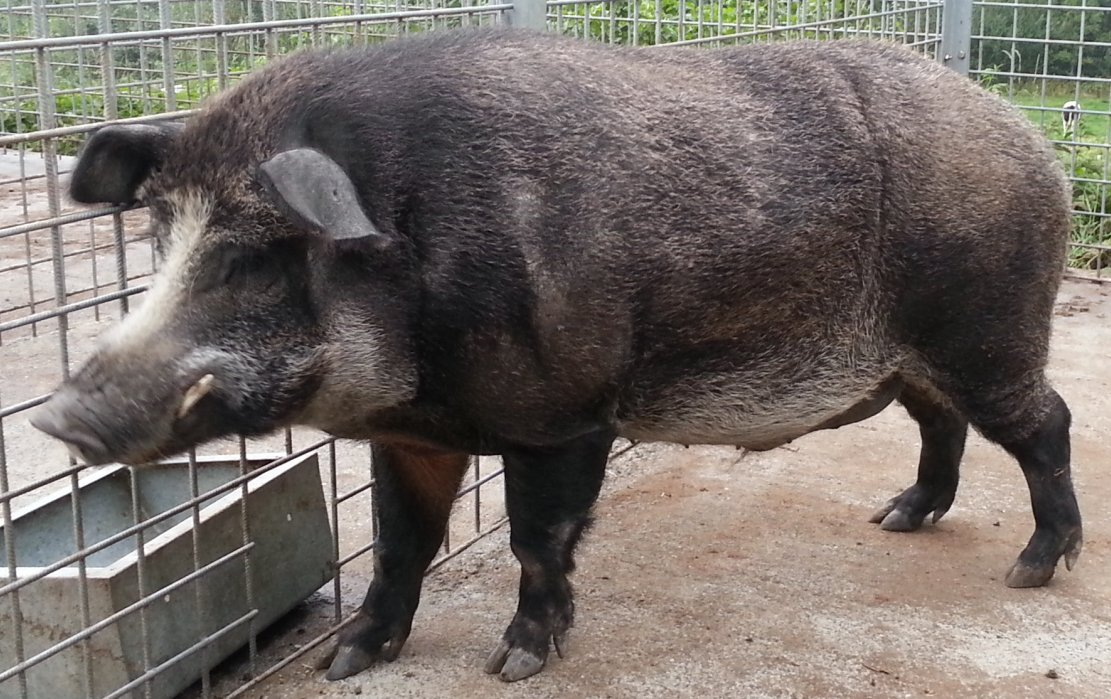
\includegraphics[scale=0.1]{javaporco.jpg}
%\end{minipage}
%
%\begin{block}{Modelo Matemático}
%Se considerarmos que uma população é extinta quando cai abaixo de um certo nível \textcolor{orange}{$m$} e que tem um valor máximo sustentável \textcolor{red}{M}, isto é, a taxa de crescimento diminui com a falta de recursos, um modelo matemático que descreve o crescimento dessa população é:
%\[\frac{dy}{dt}=ky(\textcolor{red}{M}-y)(y-\textcolor{orange}{m)}.\]
%\end{block}
%
%\footnotetext[1]{Em 2018 o javaporco foi \href{https://piaui.folha.uol.com.br/um-javaporco-no-caminho-do-governador-de-sao-paulo/}{notícia na revista piauí} por atrapalhar a campanha do candidado a governador Márcio França em SP.}
%\end{frame}
%

\begin{frame}{ }

\begin{casa}
Calcule \begin{enumerate}
\item $\dps\int\frac{2x^3-2x^2+1}{x^2-x}dx$
\item $\dps\int \frac{x^2+4x+1}{(x-1)(x+1)(x+3)}dx$
\end{enumerate}


%\begin{enumerate}
%\item $\dps \int \frac{x^2-4x-4}{x^3-2x^2+4x-8}dx$
%\item 
%\end{enumerate}

\end{casa}

\end{frame}

%\begin{frame}
%
%\begin{exer}
%Um dia em um campus universitário com 5\,000 alunos, onde se esperava uma assembleia estudantil um aluno ouviu que certo estudante polêmico iria fazer, durante a assembleia, um discurso explosivo. Essa informação foi transmitida para amigos que, por sua vez, a transmitiram a outros. A taxa com que se espalhou essa informação é conjuntamente proporcional ao número de pessoas que a ouviram e ao número de pessoas que não a ouviram. Se após 10 min 144 pessoas ouviram a informação, ache o modelo matemático que escreve a divulgação da notícia. Em quanto tempo metade das pessoas terão ouvido a notícia? 
%\end{exer}
%
%\end{frame}






\section{Aplicações da Integral}


\subsection*{Área entre curvas}


\begin{frame}{Área entre curvas}
Queremos determinar a área delimitada pelo gráfico de duas funções.



\begin{center}
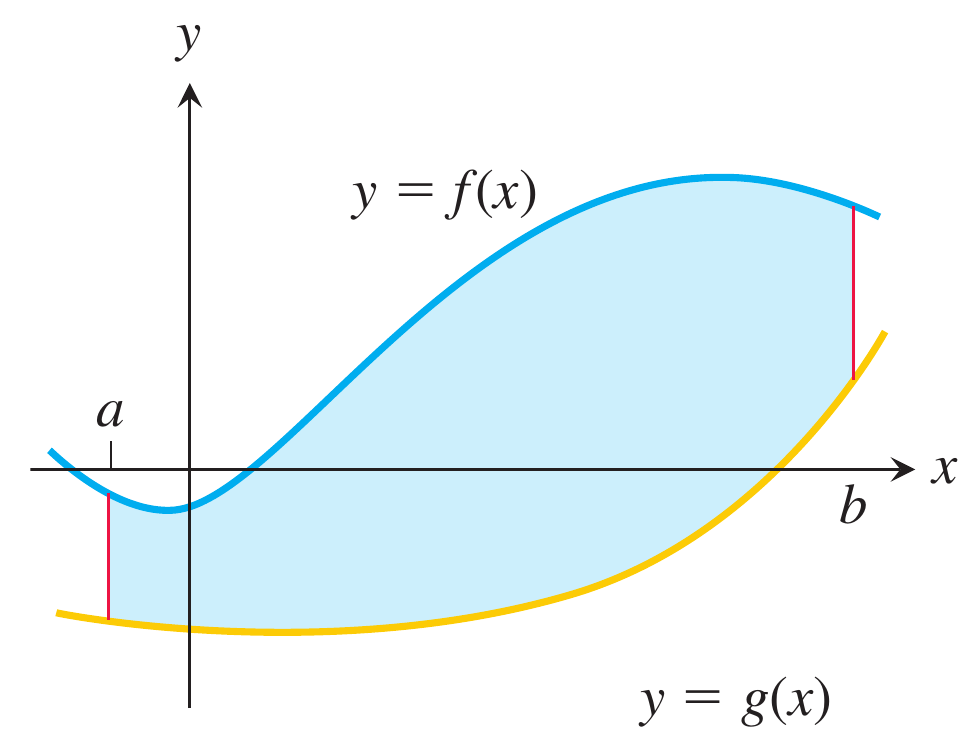
\includegraphics[scale=1]{area-curvas-th-1.png}
\end{center}
\end{frame}

\begin{frame}
No caso em que $f(x)\geq g(x)$ em $[a,b]$.

\begin{center}
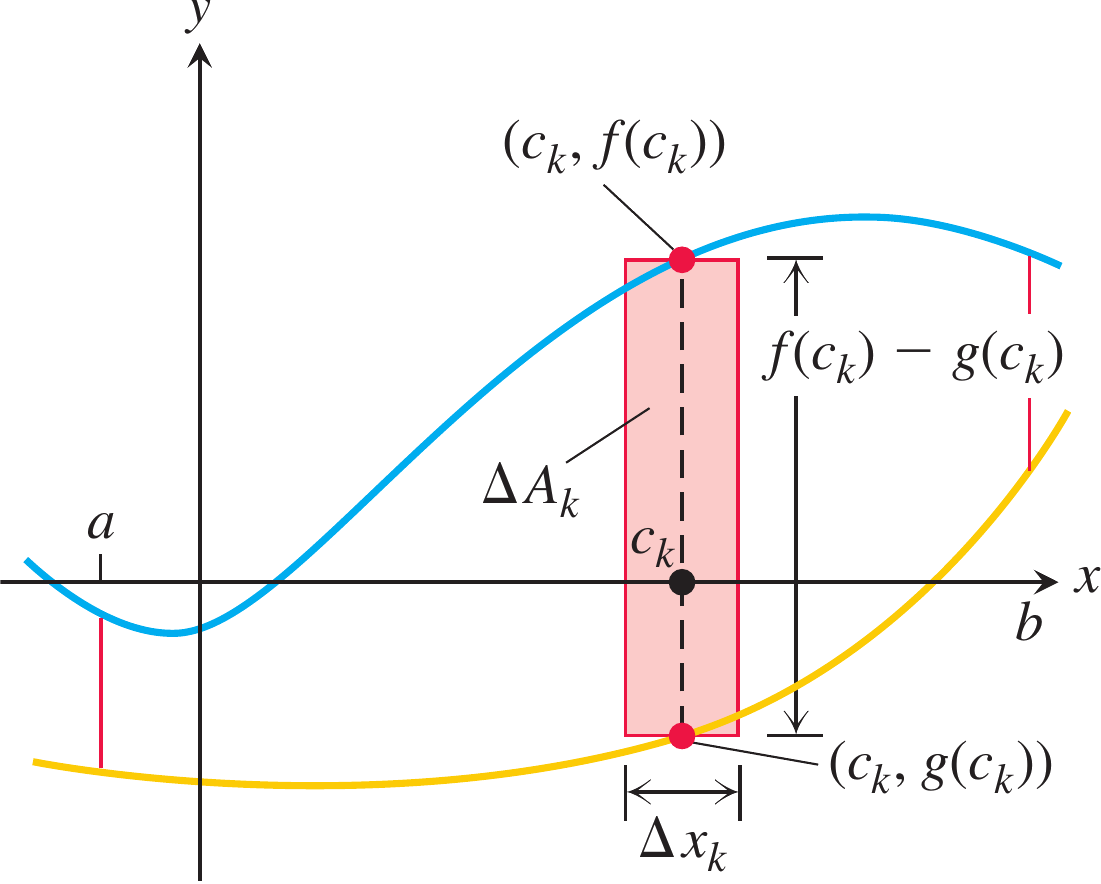
\includegraphics[scale=0.6]{area-curvas-th-3.png} \ \ \ 
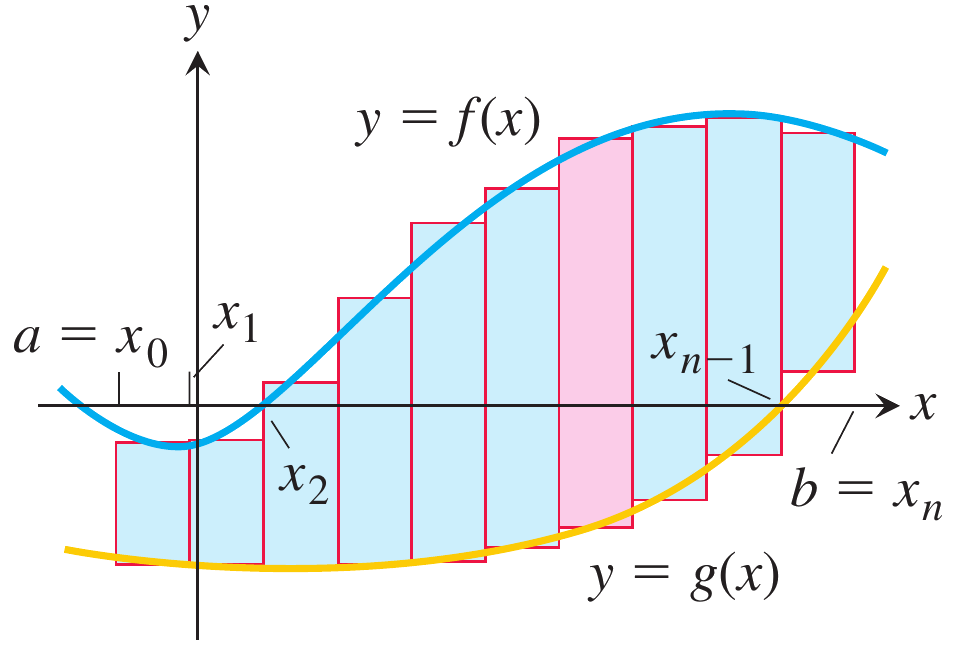
\includegraphics[scale=0.7]{area-curvas-th-2.png}
\end{center}

\[\text{Área}(S)=\lim_{\|P\|\to 0}\sum_{k=1}^{n}(f(c_k)-g(c_k))\Delta x_k=\int_a^b f(x)-g(x)dx\]
\end{frame}

%\begin{frame}
%\frametitle{Áreas entre curvas}
%%
%
%\uncover<1->{Vimos que se uma função não é negativa, então as somas de Riemann aproximam-se da área compreendida entre o gráfico da função e o eixo $OX$. Isso motiva a seguinte definição
%\begin{defin}
%Seja $f:[a,b]\to \R$ uma função integrável. A \dt{área} limitada pela curva $y=f(x)$ e o eixo $OX$ é dada por:
%$$\int_a^b|f(x)|dx$$
%\end{defin}}
%
%\begin{exe} 
% Calcule a área  limitada pela curva $y=x^2-x$ e o eixo $OX$ no intervalo $[0,2]$.
%\end{exe}
%
%%\uncover<1->{\begin{exe} 
%% Esboce o gráfico e calcule a área  limitada pela curva $y=x^3-x^2-2x$ e o eixo $OX$.
%%\end{exe}}
%
%
%\end{frame}
%
%
%\begin{frame}
%\begin{exer}
%Calcule a área limitada pela curva $y=\cos(x)$ e o eixo $OX$ no intervalo $[]$
%\end{exer}
%\end{frame}

\begin{frame}
\frametitle{Área entre curvas}



\begin{defin}
Sejam $f:[a,b]\to \R$ e $g:[a,b]\to \R$  funções integráveis. A \dt{área} limitada pelas curvas $y=f(x)$ e $y=g(x)$ e pelas retas $x=a$ e $x=b$ é dada por:
$$\int_a^b|f(x)-g(x)|dx$$
\end{defin}

\begin{center}
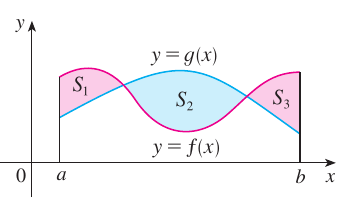
\includegraphics[scale=.7]{area-curvas.png}
\end{center}


\end{frame}

\begin{frame}

\begin{exe} 

 Determine a área limitada pelas curvas $y=2-x^2$ e $y=-x$.

%\item Determine a área entre a curva $y=x^2-1$, o eixo $x$  e as retas $x=0$ e $x=2$.

%\item Determine a área da região do primeiro quadrante que é limitada acima por $y=\sqrt{x}$ e abaixo pelo eixo $x$ e pela reta $y=x-2$.
%\end{enumerate}
\end{exe}
%
%
%\begin{exer}
%Determine a área entre as curvas $y=2x-x^2$ e $y=-3$.
%\end{exer}
%\end{frame}
%
%\begin{frame}{Integrando em relação a $y$}
As vezes é mais conveniente integrar em relação ao eixo $y$ a fim de determinar a área.

\begin{exe}
Determine a área da região do primeiro quadrante que é limitada acima por $y=\sqrt{x}$ e abaixo pelo eixo $x$ e pela reta $y=x-2$.
\end{exe}
%
%\begin{exer}
%Encontre a área da região limitada pela reta $y=x-1$ e pela parábola $y^2=2x+6$.
%\end{exer}

\end{frame}



\begin{frame}
	\begin{casa}
\begin{enumerate}
	\item Encontre a área da região limitada pelas curvas $y=\sin(x)$, $y=\cos(x)$, $x=0$ e $x=\pi/2$.
	
	\item Encontre a área da região limitada pela reta $y=x-1$ e pela parábola $y^2=2x+6$.
\end{enumerate}
	\end{casa}
\end{frame}

%\begin{frame}
%\begin{casa}
%Determine a área entre as curvas
%\begin{enumerate}
%\item $y=e^x$, $y=x$, $x=0$ e $x=1$.
%
%\item $y=x^2$ e $y=2x-x^2$
%
%\item $y=\sen x$, $y=\cos x$, $x=0$ e $x=\frac{\pi}{2}$.
%
%\item $y=x-1$ e $y^2=2x+6$.
%\end{enumerate}
%
%
%\end{casa}
%\end{frame}


\subsection*{Volume por Fatiamento}
\begin{frame}
\frametitle{Volumes por fatiamento}


Uma \dt{seção transversal } de um sólido $S$ é a região plana formada pela interseção entre $S$ e um plano. Seja $S$ um sólido limitado por dois planos perpendiculares a um eixo $OX$ nos pontos $a$ e $b$. Se $A:[a,b]\to \R$ é a função contínua que para cada $x\in[a,b]$ associa a área $A(x)$ da seção transversal de $S$ por um plano perpendicular a $OX$ no ponto $x$, então podemos aproximar o volume do sólido $S$. 

\begin{center}
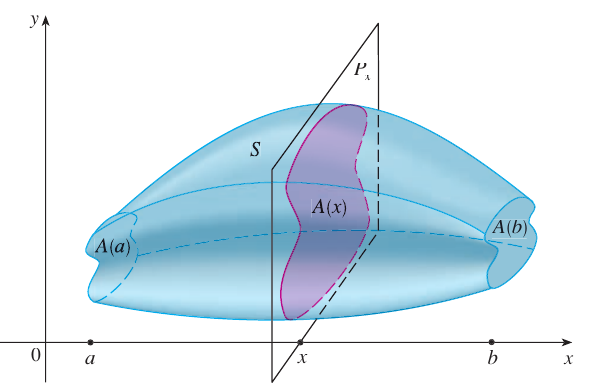
\includegraphics[scale=0.4]{volume-fatia.png}
\end{center}




\end{frame}



\begin{frame}
\begin{itemize}
\item $P=\{a=x_0,x_1,\cdots,x_n=b\}$ uma partição de $[a,b]$.
\item $S$ é divido em $n$ ``fatias'' de largura $\Delta x_k$.
\item $\{x_1^\ast,x_2^\ast,\cdots,x_n^\ast\}$ um pontilhamento da partição $P$ 
\end{itemize}

%Seja $P=\{a=x_0,x_1,\cdots,x_n=b\}$ uma partição de $[a,b]$. Os planos $P_{x_k}$ perpendiculares a $OX$ dividem $S$ em $n$ ``fatias'' de largura $\Delta x_k$. Dado um pontilhamento $\{c_1,c_2,\cdots,c_n\}$ da partição $P$ podemos ver que o volume de cada fatia $V_k$ é aproximadamente
%\[V_k\approx A(c_i)\Delta x_k.\]

\begin{center}
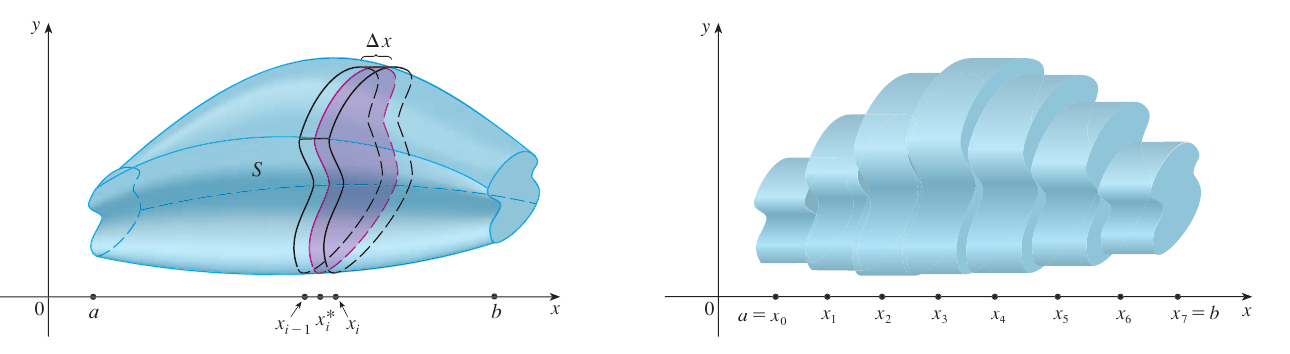
\includegraphics[scale=0.37]{volume-fatia-particao.png}
\end{center}

\[V_i\approx A(x_i^\ast)\Delta x_i.\]

\end{frame}

\begin{frame}

Portanto o volume $V$ do sólido $S$ é aproximadamente
\[V\approx\sum_{k=1}^n A(x_i^\ast)\Delta x_i.\]
Com isso, aplicando o limite quando $\|P\|\to 0$ temos que
\[V=\lim_{\|P\|\to 0}\sum_{k=1}^n A(x_i^\ast)\Delta x_i=\int_a^bA(x)dx.\] 

\end{frame}



\begin{frame}

\begin{exe}

Uma cunha curva foi obtida por meio do corte da metade de um cilindro de raio 4 por dois planos. Um deles é perpendicular ao eixo do cilindro. O segundo cruza o primeiro, formando um ângulo de $30^\circ$ no centro do cilindro. determine o volume da cunha.

\end{exe}


\begin{center}
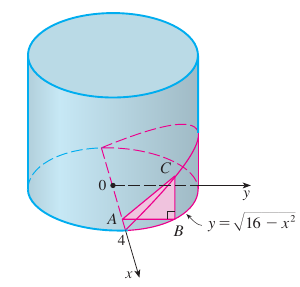
\includegraphics[scale=.7]{figuras/cunha.png}
\end{center}

\end{frame}


\subsection*{Sólidos de Revolução}
\begin{frame}{Sólidos de Revolução 
\includegraphics[scale=0.015]{figuras/fist.png}}\label{current}
\begin{center}
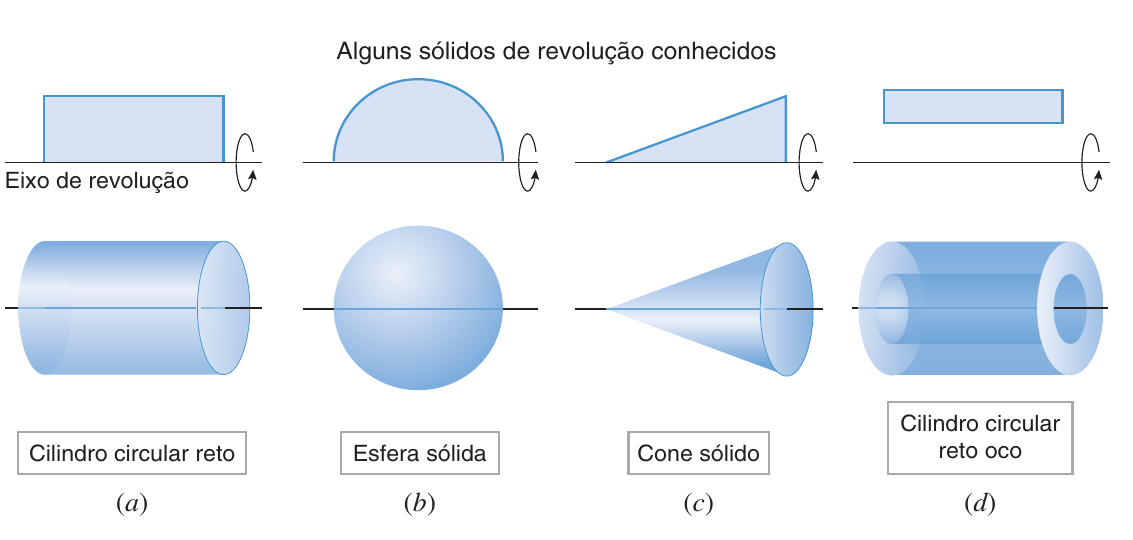
\includegraphics[scale=.4]{figuras/solidos-revolucao.png}
\end{center}
\end{frame}



\subsection*{Sólidos de Revolução: Método dos Discos}
\begin{frame}{Método dos Discos}
No caso em que o eixo de rotação é {\color{blue}paralelo} ao eixo de coordenadas, podemos usar o chamado {\color{blue} método dos discos}.

\[V=\int_a^b \pi \left(f(x)\right)^2\,dx\]

\begin{center}
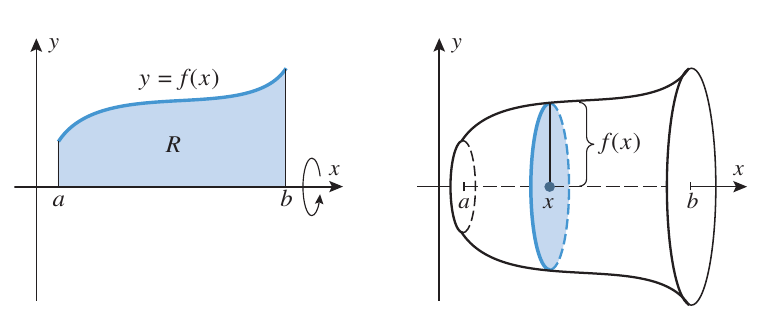
\includegraphics[scale=.4]{figuras/discos1.png}
\end{center}
\end{frame}

\begin{frame}
\begin{exe}
Mostre que o volume da esfera de raio $r$ é $\frac{4}{3}\pi r^3$.
\end{exe}

\begin{center}
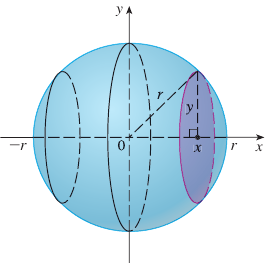
\includegraphics[scale=.7]{figuras/esfera.png}
\end{center}
\end{frame}

\begin{frame}
Usando o mesmo raciocínio, podemos resolver o seguinte tipo de problema:

\[V=\int_a^b \pi \left[\left(f(x)\right)^2-\left(g(x)\right)^2\right]\,dx\]

\begin{center}
\begin{minipage}{0.45\textwidth}
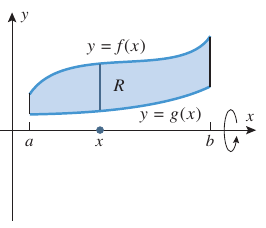
\includegraphics[scale=.5]{figuras/arruela1.png}
\end{minipage}
\begin{minipage}{0.45\textwidth}
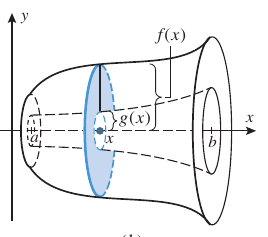
\includegraphics[scale=.5]{figuras/arruela2.png}
\end{minipage}
\end{center}
\end{frame}



\subsection*{Sólidos de revolução: Método das Cascas Cilíndricas}
\begin{frame}
\frametitle{Volume por cascas cilíndricas }
%\begin{small}

\uncover<1->{Sejam $f:[a,b]\to \R$ uma função contínua não negativa com $a>0$. Considere a região limitada pelo gráfico de $f$ e o eixo $OX$. Ao girarmos essa região em torno do eixo $OY$ geramos um sólido $S$. 

\begin{center}
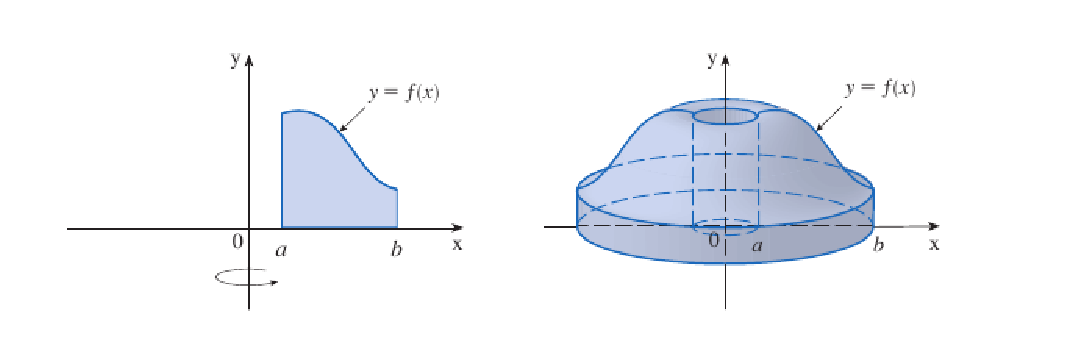
\includegraphics[scale=0.7]{casca1.eps}

\end{center}
}

%\end{small}
\end{frame}


\begin{frame}
\frametitle{ }
\begin{small}

\uncover<1->{
\begin{itemize}
\item $P=\{a=x_0,\ldots,x_n=b\}$  partição de $[a,b]$ 
\item $C=\{\overline{x}_1,\overline{x}_2,\ldots,\overline{x}_n\}$ um pontilhamento de $P$, onde $\overline{x}_i=\frac{x_{i-1}+x_i}{2}$  
\end{itemize}
\begin{center}
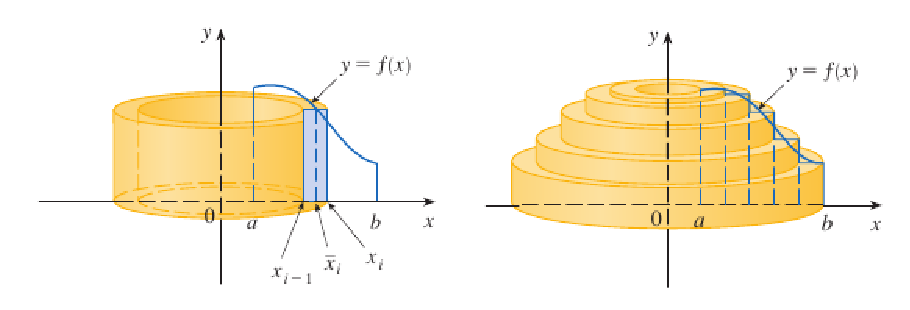
\includegraphics[scale=0.8]{casca3.eps}
\end{center} 

Com isso, o volume do sólido é dado por
$$V=2\pi\int_a^b xf(x)dx $$}

\end{small}
\end{frame}


\begin{frame}
\frametitle{ }
\uncover<1->{\begin{exe}
Calcule o volume do sólido obtido pela rotação em torno do eixo y da região limitada por $y=2x^2-x^3$ e $y=0$.

%\item Ache o volume do sólido obtido pela rotação em torno do eixo y da região entre $y=x$ e $y=x^2$.
\end{exe} }


\begin{minipage}{0.5\textwidth}
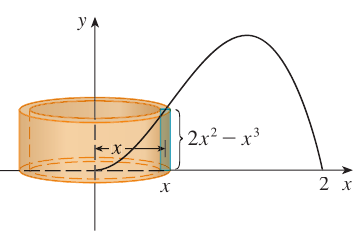
\includegraphics[scale=0.6]{figuras/solido-cascas-clindricas1.png}
\end{minipage}
\begin{minipage}{0.4\textwidth}
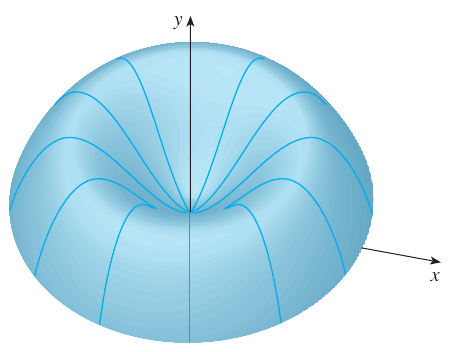
\includegraphics[scale=0.5]{figuras/solido-cascas-clindricas2.png}
\end{minipage}

\end{frame}

%\begin{frame}
%
%
%\uncover<1->{\begin{casa} Usando o método das cascas cilíndricas determine o volume do sólido gerado pela rotação da região limitada pela curva $y=\sqrt{x}$ e  pelas retas $y=1$ e $x=4$ em torno do eixo $y=-1$.
%\medskip
%
%\textbf{Resposta: $\frac{47\pi}{6}$}
%\end{casa}} 
%
%\end{frame}


\begin{frame}
\begin{casa}

\begin{enumerate}
%\item Mostre que o volume da pirâmide cuja altura é $h$ e base quadrada com lado $a$ é $\frac{1}{3}a^2h$.

\item Encontre o volume do sólido obtido pela rotação em torno do exio $x$ da região limitada  pelas curvas $y=x$ e $y=x^2$.

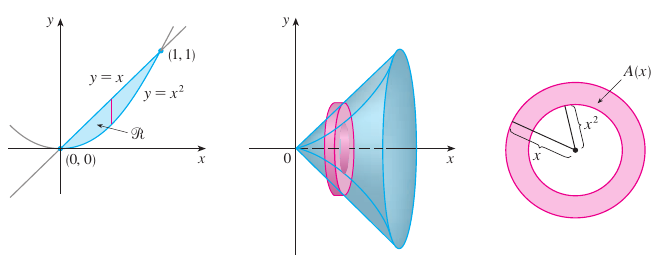
\includegraphics[scale=0.4]{figuras/arruela3.png}

\item Encontre o volume do sólido obtido pela rotação da região limitada por $y=x-x^2$ e $y=0$ em torno da reta $x=2$.

%\item Determine o volume do sólido obtido pela rotação em torno do eixo $x$ da região limitada pela curva $y=x^2+1$ e pela reta $y=-x+3$. (resposta: $117\pi/5$)
\end{enumerate}

\end{casa}
\end{frame}

\subsection*{Comprimento de Curvas}


\begin{frame}{Comprimento de Curvas}
%
\only<1>{Imagine que se queira calcular o comprimento da curva do gráfico abaixo.}
\only<2>{Uma aproximação seria o comprimento do seguimento ligando os extremos da curva.}
\only<3>{Podemos melhorar a aproximação considerando o comprimento de uma poligonal.}
\only<4>{Quanto mais divisões, melhor a aproximação!}

\begin{center}
\begin{tikzpicture}
\draw[->](0,0)--(6,0) node[below right] {$x$};
\draw[->](0,0)--(0,3)node[left] {$y$};
\draw[red,thick] plot [smooth] coordinates {(1,1)(1.5,2.3)(2,2.6)(2.5,2.3)(3,1)(3.5,1)(4,1.7)(4.5,2)(5,1.7)};

\draw<2>[blue] (1,1) -- (5,1.7);

\draw<3>[blue](1,1)--(2.5,2.3)--(5,1.7);

\draw<4>[blue] (1,1)--(1.5,2.3)--(2,2.6)--(2.5,2.3)--(3,1)--(3.5,1)--(4,1.7)--(4.5,2)--(5,1.7);
\end{tikzpicture}
\end{center}
%
%
\end{frame}
%


\begin{frame}


Assim, seja \textcolor{red}{$f:[a,b]\to \R$} uma função, a fim de calcular uma aproximação do comprimento da curva dada pelo gráfico de $f$ subdividimos o intervalo $[a,b]$ em vários subintervalos e calculamos o comprimento da \textcolor{blue}{poligonal}, como abaixo.

\begin{center}
\begin{tikzpicture}
\draw[->](0,0)--(6,0) node[below right] {$x$};
\draw[->](0,0)--(0,3)node[left] {$y$};
%\psdots(1,0)(5,0)
\draw[red,thick] plot [smooth] coordinates {(1,1)(1.5,2.3)(2,2.6)(2.5,2.3)(3,1)(3.5,1)(4,1.7)(4.5,2)(5,1.7)};
\draw[blue] plot [mark=*,mark size=1] coordinates {(1,1)(1.5,2.3)(2,2.6)(2.5,2.3)(3,1)(3.5,1)(4,1.7)(4.5,2)(5,1.7)};
%\draw[blue] (1,1)--(1.5,2.3)--(2,2.6)--(2.5,2.3)--(3,1)--(3.5,1)--(4,1.7)--(4.5,2)--(5,1.7);
\draw[dashed](2.5,0)--(2.5,2.3)--(0,2.3);
\draw[dashed](3,0)--(3,1)--(0,1);
%\psdots(1,0)(1.5,0)(2,0)(2.5,0)(3,0)(3.5,0)(4,0)(4.5,0)(5,0)(0,2.3)(0,1)
\draw[dashed] (1,0) -- (1,1);
\draw[dashed] (5,0) -- (5,1.7);
\node at (0.9,-0.3) {$a$};
\node at(4.9,-0.3){$b$};
\node[scale=0.8] at(2.4,-0.3){$x_{i-1}$};
\node[scale=0.8] at(3,-0.3){$x_{i}$};
\node at(-1,2.3){$f(x_{i-1})$};
\node at(-0.7,1){$f(x_i)$};
\end{tikzpicture}
\end{center}

\[L_i=\sqrt{\Delta x_i^2+(f(x_i)-f(x_{i-1}))^2}=\sqrt{1+\left(\frac{f(x_i)-f(x_{i-1})}{\Delta x_i}\right)^2}\ \Delta x_i\]

\end{frame}
%
%
%
\begin{frame}
\frametitle{ }


Pelo Teorema do Valor Médio, existe $c_i\in [x_{i-1},x_i]$ tal que 
\[\dps\frac{f(x_i)-f(x_{i-1})}{\Delta x_i}=f'(c_i),\]
portanto,
\[L_i=\sqrt{1+(f'(c_i))^2}\ \Delta x_i\]

Com isso, o comprimento $L$ da curva é 
\[L=\lim_{\|P\|\to 0} \sum_{i=1}^n\sqrt{1+(f'(c_i))^2}\ \Delta x_i=\int_a^b\sqrt{1+(f'(x))^2}\ dx.\]

\end{frame}

\begin{frame}



\begin{exe}\begin{enumerate}
\item Calcule o comprimento de arco da curva $y =\sqrt{x^3} $ entre os pontos $(1, 1)$ e $(4, 8)$.

\item Mostre que o comprimento da circunferência de um círculo de raio $r$ é $2\pi r$. 

%\item Calcule o comprimento de arco da curva $y=\frac{x^4}{4}+\frac{1}{8x^2}$ tal que $1\leq x\leq 2$.

%\item Calcule o comprimento de arco da catenária $y=\cosh x$ no intervalo $[-1,1]$.

\end{enumerate}
\end{exe}
\end{frame}






\section*{Integrais Impróprias}


\subsection*{Intervalo Infinito}
\begin{frame}
\frametitle{ Integrais Impróprias: Intervalo Infinito}
% 

\uncover<1->{Vimos que a integral definida de uma função {\color{blue}positiva} representa a área abaixo de seu gráfico. Analisando o gráfico da função $\dps\frac{1}{x^2}$ quando $x\in[1,+\infty)$ somos levados a pensar que a região sob o gráfico tem {\color{red}área ``infinita''}. }
\bigskip

Sabemos que 
 \[\int\frac{1}{x^2}dx=-\frac{1}{x}+c. \]
 Porém não faz sentido aplicar o Teorema Fundamental do Cálculo.
 \bigskip
 
 
% 
\end{frame}

\begin{frame}[label=improprias]
Entretanto, para cada $t\in(0,1)$ podemos calcular 
 \[\int_1^t\frac{1}{x^2}dx=1-\frac{1}{t}.\]   
 \begin{center}
 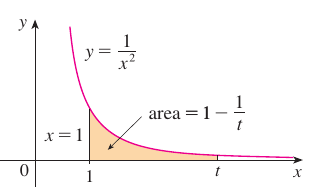
\includegraphics[scale=.7]{impropria1.png}
 \end{center}
Portanto faz sentido aplicar o limite quanto $t\to +\infty$ e podemos definir a {\color{red} área da região} por
\[\int_1^\infty \frac{1}{x^2}\, dx=\lim\limits_{t\to+\infty} \int_1^t\frac{1}{x^2}\, dx=\lim\limits_{t\to \infty} \left(1-\frac{1}{t}\right)=1.\]
\end{frame}



\begin{frame}[label=improprias]
\frametitle{ }
 

\uncover<1->{\begin{defin} \begin{enumerate}[a]
\item Se $\dps\int_a^{{\color{red} b}} f(x)dx$ existe para cada número ${{\color{red}b}}\geq a$, então definimos
\[\int_a^{{\color{red}+\infty}}f(x)dx:=\lim_{{\color{red}b\to+\infty}}\int_a^{{\color{red} b}} f(x)dx.\]


\item Se $\dps\int_{{\color{red}a}}^b f(x)dx$ existe para cada número ${\color{red}a}\leq b$, então definimos
\[\int_{{\color{red}-\infty}}^{b}f(x)dx:=\lim_{{\color{red}a\to -\infty}}\int_{{\color{red}a}}^b f(x)dx.\]


As integrais acima são ditas \dt{impróprias}. Se os limites existem dizemos que as integrais impróprias {\color{blue}convergem} e  se os limites não  existem dizemos que elas {\color{red}divergem}.

\end{enumerate}
\end{defin} }

 
\end{frame}

\begin{frame}
\frametitle{ }
 

\uncover<1->{\begin{defin} Se $\dps \int_{-\infty}^{b}f(x)dx$ e $\dps \int_b^{+\infty}f(x)dx$ são convergentes, então definimos
$$\int_{-\infty}^{+\infty}f(x)dx=\int_{-\infty}^{b}f(x)dx+ \int_b^{+\infty}f(x)dx$$

\end{defin} }



\uncover<1->{\begin{exe}\begin{enumerate}[a]
\item Calcule $\dps\int_{-\infty}^0xe^xdx$

\item Calcule $\dps\int_{-\infty}^{+\infty}\frac{1}{1+x^2}dx$

\end{enumerate}
\end{exe}}

 
\end{frame}



\begin{frame}[label=improprias]
\begin{casa}
 \begin{enumerate}
 \item Determine os valores de $p\in \R$ para os quais a seguinte integral converge
 \[\int_1^{+\infty}\frac{1}{x^p}dx\]
 
 
 \item Calcule o volume do sólido de revolução gerado pela rotação da curva $y=\frac{1}{x}$, quando $1\leq x<+\infty$, em torno do eixo $x$, conhecido como \dt{Trombeta de Gabriel} ou \dt{Trombeta de Torricelli}
 
 
 \begin{center}
 
\includegraphics[scale=0.1]{GabrielHorn}
 \end{center}

 \end{enumerate} 
\end{casa}
\end{frame}




\subsection*{Integrando Descontínuo}
\begin{frame}
\frametitle{Integrais Impróprias: Integrando Descontínuo}
% 

Agora, suponha que queremos calcular a área abaixo do gráfico da função $\dps f(x)=\frac{1}{x^2}$ quando $x\in{\color{red}(0},1]$. Sabemos que 
 \[\int\frac{1}{x^2}dx=-\frac{1}{x}+c. \]
 Porém não faz sentido aplicar o Teorema Fundamental do Cálculo, pois a função não está definida em {\color{red}$x=0$}.
\bigskip

De modo análogo ao feito anteriormente, podemos definir a área da seguinte forma
\[\int_{{\color{red}0}}^{1}\frac{1}{x^2}\,dx=\lim_{{\color{red}t\to 0^+}}\int_{{\color{red}t}}^1\frac{1}{x^2}\,dx=\lim_{{\color{red}t\to 0^+}}\left(-1+\frac{1}{t}\right)=+\infty.\]



% 
\end{frame}





\begin{frame}
\frametitle{ }
 

\uncover<1->{\begin{defin} \begin{enumerate}[a]
\item Se $f$ é contínua em $({\color{red}a},b]$ e descontínua em {\color{red}$a$}, então definimos
\[\int_{{\color{red}a}}^b f(x)dx:=\lim_{t\to {\color{red}a^+}}\int_t^b f(x)dx.\]


\item  Se $f$ é contínua em $[a,{\color{red}b})$ e descontínua em {\color{red}$b$}, então definimos
\[\int_a^{{\color{red}b}} f(x)dx:=\lim_{t\to {\color{red}b^-}}\int_a^t f(x)dx.\]


\item  Se $f$ é contínua em $[a,{\color{red}c})\cup({\color{red}c},b]$ e descontínua em {\color{red}$c$}, então definimos
\[\int_a^b f(x)dx:=\int_a^{{\color{red}c}} f(x)dx+\int_{{\color{red}c}}^b f(x)dx.\]

\end{enumerate}
\end{defin} }

 
\end{frame}


\begin{frame}
\frametitle{ }
 

\uncover<1->{\begin{exe}\begin{enumerate}
\item Calcule $\dps\int_{2}^5\frac{dx}{\sqrt{x-2}}$

\item Calcule $\dps\int_0^3\frac{1}{x-1}dx$.

\end{enumerate}
\end{exe} }

\begin{casa}
Calcule 
\[\int_0^1 \log(x)\, dx.\]
\end{casa}


 
\end{frame}


\begin{frame}
\frametitle{Trombeta de Gabriel}
 

\uncover<1->{Podemos encontrar em livros de cálculo que a área de uma superfície gerada pela rotação, em torno do eixo x, do gráfico de uma função $f$ não-negativa definida em $[a,b]$  é dada por
\[S=\int_a^b 2\pi f(x)\sqrt{1+(f'(x))^2}\ dx\]
Com isso temos que a área de superfície da {\color{blue}Trombeta de Gabriel} é dado pela integral 
\[\dps\int_1^{+\infty}2\pi \frac{1}{x}\sqrt{1+\frac{1}{x^4}}dx.\]
}
\end{frame}

\begin{frame}
Note que $\sqrt{1+\frac{1}{x^4}}>1,\ \forall x>0$. Com isso,
\[\int_1^b2\pi \frac{1}{x}\sqrt{1+\frac{1}{x^4}}dx\geq\int_1^b 2\pi \frac{1}{x}dx.\]



\begin{center}

\includegraphics[scale=0.1]{trombeta.eps}
\end{center}

Aplicando o limite deduzimos que a primeira integral diverge. Assim, a trombeta do Anjo Gabriel tem {\color{blue}volume finito} porém {\color{red} área de superfície infinita}, ou seja, O arcanjo poderia encher a trombeta com pouco mais de 3 unidades cúbicas de tinta, mas mesmo que usasse toda a tinta do universo, não poderia pintá-la!!! 

 
\end{frame}


\begin{frame}
\frametitle{ Teste de comparação  }
 

\uncover<1->{Algumas vezes é impossível ou uma tarefa muito difícil calcular o valor exato de uma integral imprópria, mas ainda assim é importante saber se ela é convergente ou divergente

\begin{teo}[Teste de comparação]
Suponha que $f$ e $g$ sejam funções contínuas com ${\color{red}0\leq }\, g(x)\leq f(x)$ para $x\geq a$.
\begin{enumerate}[a]
\item Se $\dps\int_a^b f(x)dx$ é {\color{blue}convergente}, então $\dps\int_a^b g(x)dx$ também {\color{blue}convergente}.
\item Se $\dps\int_a^b g(x)dx$ é {\color{red}divergente}, então $\dps\int_a^b f(x)dx$ também {\color{red}divergente}.
\end{enumerate}
\end{teo}. }

\uncover<1->{O teste também é válido quando um dos extremos do limite de integração é infinito.}



 
\end{frame}


\begin{frame}
\frametitle{ }
 

\uncover<1->{\begin{exe}Decida sobre a convergência das integrais.\begin{enumerate}[a]
\item $\dps \int_1^{\infty}e^{-x^2}dx$
\item $\dps \int_0^{1}\frac{dx}{\sqrt{x+x^3}}$
\end{enumerate}
\end{exe}}



 
\end{frame}



\begin{frame}
\frametitle{Teste de comparação no limite }
 

\uncover<1->{\begin{teo}
Sejam $f$ e $g$  funções \textcolor{red}{positivas} e contínuas em $[a,+\infty)$ tais que
$$\lim_{x\to+\infty}\frac{\textcolor{red}{f(x)}}{\textcolor{blue}{g(x)}}=L.$$
\begin{enumerate}[$i$]
\item Se $0<L<+\infty$, então
as integrais $\dps\textcolor{red}{\int_a^{+\infty}f(x)dx}$ e $\dps\textcolor{blue}{\int_a^{+\infty}g(x)dx}$ são ambas convergentes ou ambas divergentes.
 
 \item Se $L=0$ e $\dps\textcolor{blue}{\int_a^{+\infty}g(x)dx}$ converge, então 
 $\dps\textcolor{red}{\int_a^{+\infty}f(x)dx}$ também converge.
 
\end{enumerate}

\end{teo}}



 
\end{frame}

\begin{frame}
\begin{obs}\begin{enumerate}
\item Se $\dps\lim_{x\to+\infty}f(x)=+\infty$, então  $\dps\int_a^{+\infty}f(x)dx$ diverge.
\item Este teste também é válido para os outros tipos de integrais impróprias, mutatis mutandis.
\end{enumerate}

\end{obs}
\end{frame}



\begin{frame}
\frametitle{ }
 

\uncover<1->{\begin{prop} Seja $f$ contínua em $[a,b)$. Se $\dps\int_a^b|f(x)|dx$ converge, então $\dps\int_a^b f(x)dx$ também converge.
\end{prop}}

\uncover<2->{\begin{exe} Decida sobre a convergência da integrais.
\begin{enumerate}
\item  $\dps \int_1^{+\infty}\frac{dx}{\sqrt{2x^2+5x^3}}$
\item $\dps\int_1^{+\infty}\frac{\sen x}{x^3}dx$
\item $\dps \int_1^{+\infty}\frac{x}{\cosh x}dx$
\end{enumerate}
\end{exe} }

 
\end{frame}





\end{document}



\begin{frame}
\frametitle{ }
\begin{scriptsize}

\uncover<1->{ }

\end{scriptsize}
\end{frame}
